\section{Numerical study}\label{sec:blup:numerical_study} 
%In this section, we present a finite-sample Monte Carlo simulation study and a real data application using national electricity consumption and production data for France, available on the ODR\'E platform \citep{odre_data}. We consider daily consumption curves as well as photovoltaic and hydroelectric production curves. First, the consumption curves are used to estimate the parameters of a first-order autoregressive process (FAR(1)), which are then used to generate new curves for the Monte Carlo simulations. Second, for the real data application, we apply our methods directly to each type of curve. The results were obtained using the R package \texttt{adaptiveFTS} and additional code, both publicly available at \url{https://github.com/hmaissoro}. An Epanechnikov kernel ($K(u) = (3/4)(1-u^2)$ for $|u|\leq 1$, and $0$ otherwise) is used in all experiments.

In this section, we present a finite-sample Monte Carlo simulation study and a real data application. The simulation study is based on national electricity consumption curves for France, available from the ODR\'E platform \citep{odre_data}. These curves are used to estimate the parameters of a first-order autoregressive process (FAR(1)), which are then used to generate synthetic curves for the Monte Carlo simulations. For the real data application, we analyse daily Facebook stock volume curves, available at \url{https://firstratedata.com/}. All results were obtained using the \texttt{R} package \texttt{adaptiveFTS} and supplementary code, both of which are publicly available at \url{https://github.com/hmaissoro}. An Epanechnikov kernel ($K(u) = (3/4)(1 - u^2)$ for $|u| \leq 1$, and $0$ otherwise) is used in all experiments.


 

\subsection{Simulation setting}\label{blup:sec:simu_exp}
The Monte Carlo simulation is based on France's daily national electricity consumption curves from June to September 2024. The dataset contains 122 curves, one for each day within this period. Each curve represents electricity consumption recorded at 96 evenly spaced time points throughout the day, with measurements taken every 15 minutes. For readability, we normalise the curves to the interval $[0,1]$ by dividing each value by the maximum consumption observed over the entire period. Figure~\ref{fig:conso_last_curves} displays the last four consumption curves from the dataset. 

To simulate FTS with patterns similar to those of the observed curves, we estimate the parameters of a FAR(1) model from the data and use them to generate synthetic FTS samples. We consider the FAR(1) process with an associated innovation process $\{\xi_n\}$, defined as:
\begin{equation}\label{blup:FTS_mod1}
	X_n(u) = \mu(u) + \int_0^1\psi(u,s)(X_{n-1}(s)-\mu(s))\,ds + L_t\xi_n(u),
\end{equation}
where the mean function $\mu$ and the kernel of the autoregressive operator $\psi$ are estimated from the real consumption curves. The innovation process $\{\xi_n\}$ is independently generated as a multi-fractional Brownian motion, with the Hurst index function also estimated from the real consumption curves \citep[see][]{taqqu2006}. Let us note that, as shown in Example 2 of \citet{Maissoro2025}, if the kernel $\psi(\cdot,s)$ is Hölder continuous with a Hölder exponent greater than the regularity of $\{\xi_n\}$, then the FTS $\{X_n\}$ inherits the regularity of the innovation process. In particular, $\{X_n\}$ has a local Hölder exponent corresponding to the Hurst index function of $\{\xi_n\}$ and a Hölder constant $L_t^2$.


The estimation procedure for $\mu$ and $\psi$ using Fourier expansion is detailed in the supplementary material of \citet{Maissoro2025}. The local Hölder exponent is estimated from the real dataset using the local regularity estimators proposed by \citet{Maissoro2025} over a grid of points and smoothed using natural cubic splines. Figure~\ref{fig:simu_param} shows the estimated local exponent $\widehat{H}_t$, along with the estimated mean function $\mu$ and the autoregressive kernel $\psi$, where the kernel norm is normalised to $0.5$.

\begin{figure}[t!]
	\centering
	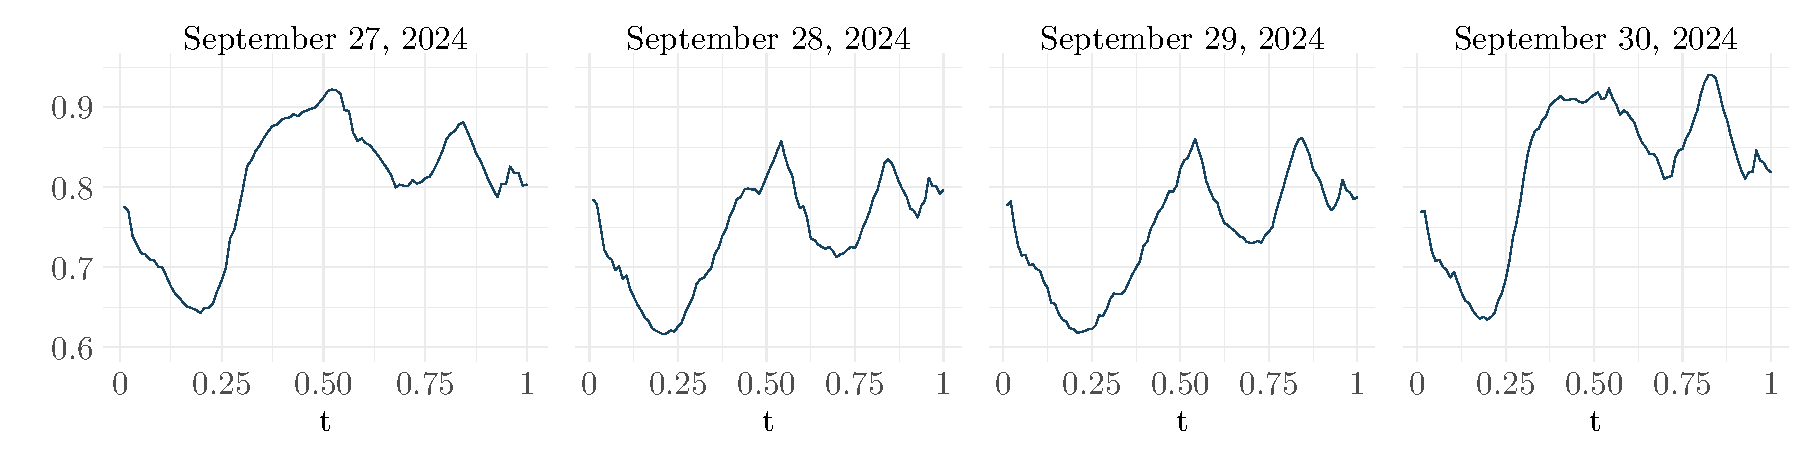
\includegraphics[width=\textwidth]{./figures/real_data_conso_4last_curves.pdf}
	\caption{\small The last four daily national electricity consumption curves in France from the dataset, with values normalised to the interval $[0,1]$.}
	\label{fig:conso_last_curves} 
\end{figure}

\begin{figure}[h!]
	\centering
	\begin{tabular}{ccc}
		\small (a) $\footnotesize \widehat{H}_t$ for simulation & \small (b) $\footnotesize \widehat{\mu}$ for simulation & \small (c) $\footnotesize \widehat{\psi}$ for simulation\\
		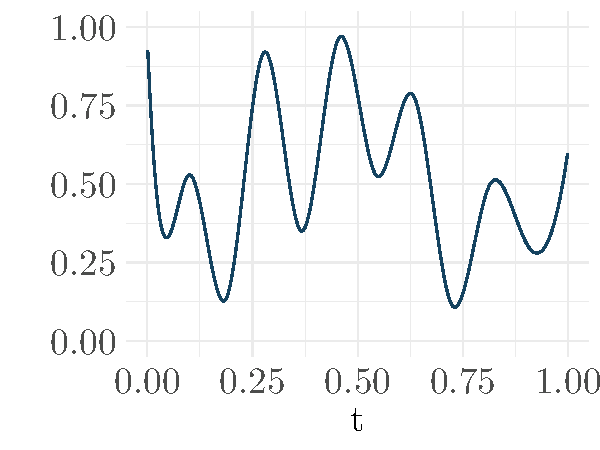
\includegraphics[width=0.3\textwidth]{./figures/local_exponent_conso.pdf} & 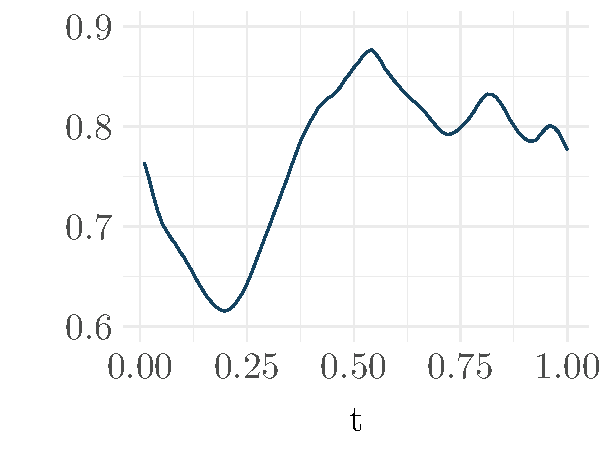
\includegraphics[width=0.3\textwidth]{./figures/smooth_mean_conso.pdf} &
		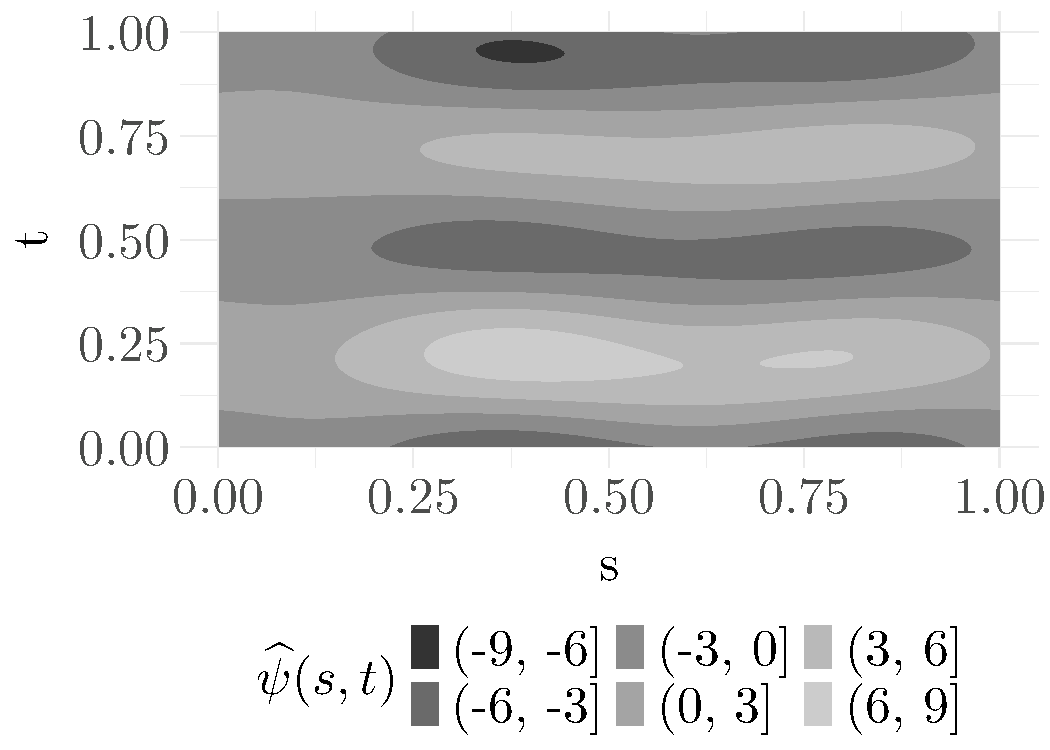
\includegraphics[width=0.3\textwidth]{./figures/far_kernel_conso.pdf}
	\end{tabular}
	\caption{\small Simulation parameters estimated from consumption curves: (a) estimated local exponent function, (b) estimated mean function, (c) estimated autoregressive kernel.}
	\label{fig:simu_param}
\end{figure}

To obtain the data points according to \eqref{eq:model}, the number of points on each curve, $M_n$, is randomly generated from a uniform distribution between $0.8\lambda$ and $1.2\lambda$, while the observation times $\{T_{n,i}\}$ are drawn independently from a uniform distribution on the interval $(0,1]$. We set $L_t = 0.1$, corresponding to the mean of the estimates of the local Hölder constant of the consumption curves, evaluated over an equidistant grid of $99$ points between $0.01$ and $0.99$, and obtained using the estimator proposed by \citet{Maissoro2025}. For the observation error term, we set $\sigma(T_{n,i}) = 0.007$, corresponding to the mean standard deviation of the consumption curves estimated using \eqref{eq:blup:sigma_estimator} over the observation grid, and the $\varepsilon_{n,i}$ are centred Gaussian variables with unit variance. A sequence of $100$ burn-in steps is used to initialise \eqref{blup:FTS_mod1}. Figure~\ref{fig:generated_last_curves} illustrates the simulated sample paths and the randomly observed points for a sample size of $(N, \lambda) = (150, 25)$.      


\begin{figure}[t!]
	\centering
	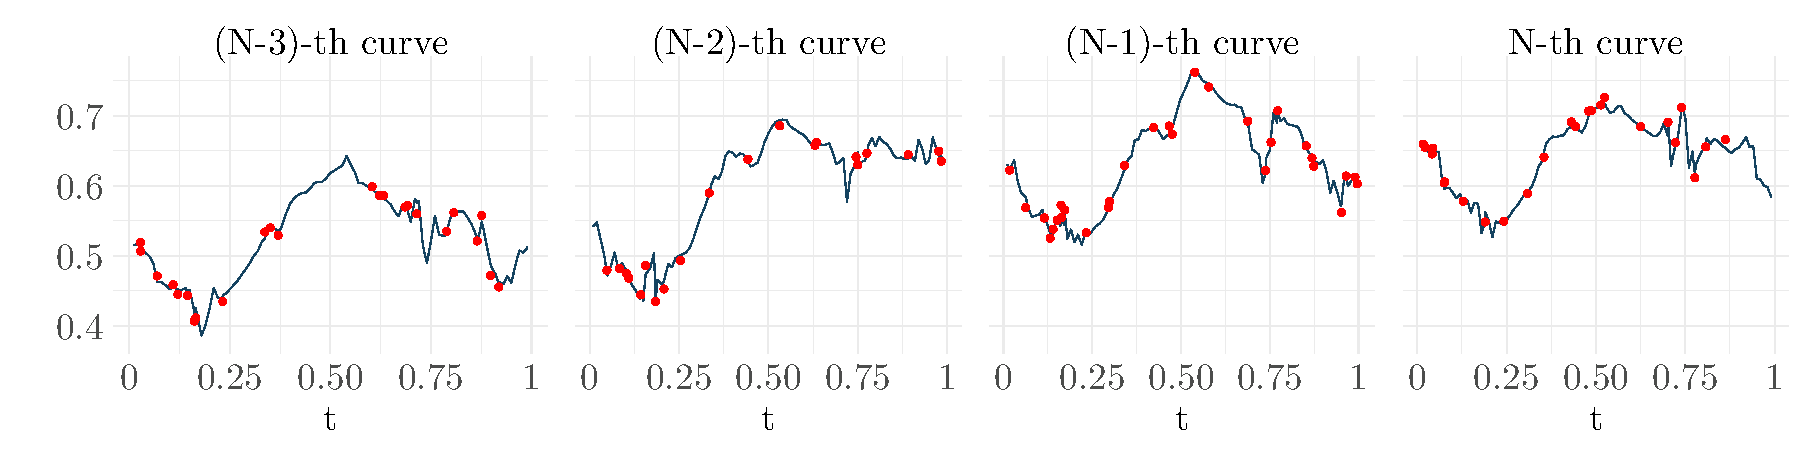
\includegraphics[width=\textwidth]{./figures/generated_conso_4last_curves.pdf}
	\caption{\small Last four simulated curves generated using the simulation setting with a sample size of $(N, \lambda) = (150, 25)$. The solid lines represent the sample paths, while the dots indicate the randomly observed noisy points on each curve, with an average of $\lambda = 25$ points per curve.}  
	\label{fig:generated_last_curves} 
\end{figure}

Finally, for the (auto)covariance study we generate different samples of FTS, whereas for the BLUP study we generate a single sample of FTS and regenerate its last curve. The aim of the (auto)covariance study is to show that the proposed method performs at least as well as the approach of \cite{Maissoro2025}, which uses a single bandwidth. Meanwhile, the aim of the BLUP study is to show that a curve, here the last curve, is accurately reconstructed.

\begin{figure}[h!]
	\centering
	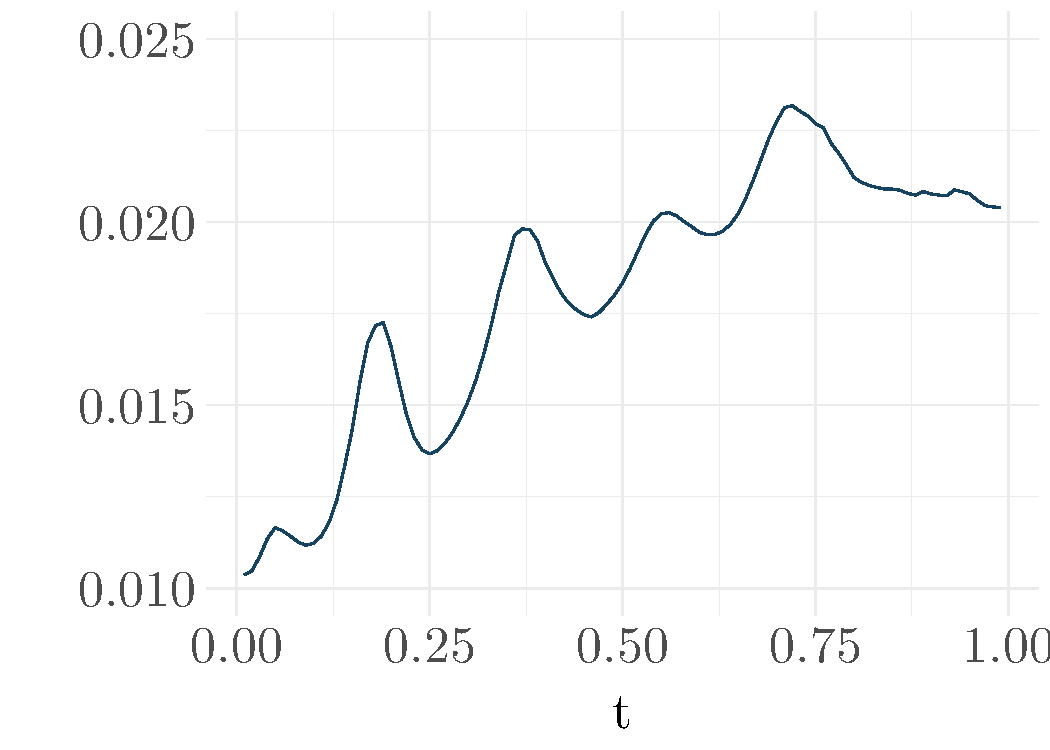
\includegraphics[width=0.4\textwidth]{./figures/variance_FTS_new_design_conso_lag=0.pdf} 
	\caption{\small Variance of the constructed FTS process from \eqref{blup:FTS_mod1} and the consumption curves.}
	\label{fig:var_FTSConso}
\end{figure}


\subsection{Implementation details}
The estimation of the lag-$\ell$, $\ell \geq 0$, (auto)covariance using the estimators in \eqref{eq:hat_Gamma_ell}, \eqref{eq:hat_Gamma_0:diagonal_outside}, and \eqref{eq:hat_Gamma_0:diagonal} involves selecting optimal bandwidths based on the data-driven rules given in \eqref{eq:gamma:risk-minimization}, \eqref{eq:gamma_0:diagonal_outside:risk-minimization}, and \eqref{eq:gamma_0_diag:risk-minimization}, respectively. Computing $\widehat{R}_{\Gamma_\ell}$ requires estimating the dependence coefficients $\mathbb{D}_\ell(s, t; h_s, h_t)$, $\mathbb{D}_\ell(t,h_t|s,h_s)$, and $\mathbb{D}(t; h_t)$, which is computationally intensive.
To reduce computation time, we adopt a simplified approach. Let $\widetilde{X}_n$ denote the NW estimator of the curve $X_n$, obtained using a bandwidth selected via cross-validation. Given a set of sample points $\{(Y_{n,1}, T_{n,1}), \ldots, (Y_{n,M_n}, T_{n,M_n})\}$ for a curve $X_n$, the cross-validated optimal bandwidth for the estimator in \eqref{eq:blup:LP_est_v} is defined as
\begin{equation}\label{eq:NW_bw_cv}
	h^* \in \argmin_h \sum_{i = 1}^{M_n}\left\{Y_{n,i} - \widetilde{X}_n^{(-i)}(T_{n,i};h)\right\}^2,
\end{equation}
where $\widetilde{X}_n^{(-i)}(T_{n,i};h)$ denotes the estimator in \eqref{eq:blup:LP_est_v} computed without the $i$-th observation and using bandwidth $h$. Moreover, let $\widetilde{Z}_n(t) = \widetilde{X}_n(t) - \widetilde{\mu}_N(t)$, and define, for all $s, t \in I$,
\begin{equation*}
	\widetilde{\mu}_N(t) = \frac{1}{N} \sum_{n=1}^{N} \widetilde{X}_{n}(t), \qquad
	\widetilde{\Gamma}_\ell(s, t) = \frac{1}{N - \ell} \sum_{n = 1}^{N - \ell} \widetilde{Z}_n(s) \widetilde{Z}_{n + \ell}(t), \quad \ell \geq 1.
\end{equation*}
Then, instead of estimating $\mathbb{D}_\ell(s, t; h_s, h_t)$, $\mathbb{D}_\ell(t,h_t|s,h_s)$, and $\mathbb{D}(t; h_t)$, we simply consider the following 
\begin{multline}
	\widehat{\mathbb{D}}_\ell(s,t;h_s, h_t) 
	= \frac{1}{N-\ell} \sum_{n=1}^{N - \ell} \left\{\widetilde{Z}_n(s) \widetilde{Z}_{n + \ell}(t) - \widetilde{\Gamma}_\ell (s,t)\right\}^2 \\
	+ \!\!\!\!\sum_{k = 1}^{N-\ell - 1}\frac{2 P_{N,\ell}^{-1}(s, t; h_s, h_t)}{N - \ell - k} \Biggl|\sum_{n = 1}^{N - \ell - k - 1}\!\left\{\widetilde{Z}_n(s) \widetilde{Z}_{n + \ell}(t) - \widetilde{\Gamma}_\ell (s,t)\right\} \left\{\widetilde{Z}_{n + k}(s) \widetilde{Z}_{n + \ell + k}(t) - \widetilde{\Gamma}_\ell (s,t)\right\}\!\Biggr|,
\end{multline}
\begin{multline}
	\widehat{\mathbb{D}}_\ell(t,h_t|s,h_s)  = 24 \!\!\!\!\!\!\!\!\!\!\!\!\!\!\!\!\!\sum_{1\leq n_1<n_2<n_3\leq \ell_{\max}}\!\!\!\!\!\!\!\!\!\!\!\!\!\!\!\!(N - n_3)^{-1}\left|\sum_{k=1}^{N - n_3} \!\! \frac{p_{k,n_1, n_2}(t;h_t)}{P_{N,\ell}^{3}(s, t; h_s, h_t)} \left\{\widetilde{Z}_k \widetilde{Z}_{k + n_1} \widetilde{Z}_{k + n_2} \widetilde{Z}_{k + n_3}\right\}(t) \right| \\
	+ 6 \!\!\!\!\!\!\!\!\!\!\!\!\!\!\sum_{1\leq n_1<n_2\leq \ell_{\max}} \!\!\!\!\!\!\!\!\!\!\!\!\!(N - n_2)^{-1}\left|\sum_{k=1}^{N - n_2} \! \frac{p_{k,n_1, n_2, n_3}(t;h_t)}{P_{N,\ell}^{3}(s, t; h_s, h_t)} \left\{\widetilde{Z}_k^2 \widetilde{Z}_{k + n_1} \widetilde{Z}_{k + n_2} + \widetilde{Z}_k \widetilde{Z}_{k + n_1}^2 \widetilde{Z}_{k + n_2} + \widetilde{Z}_k \widetilde{Z}_{k + n_1} \widetilde{Z}_{k + n_2}^2\right\}(t)\right|,
\end{multline}
\begin{multline}
	\widehat{\mathbb{D}}(t; h_t)  = 24 \!\!\!\!\!\!\!\!\!\!\!\!\!\!\!\!\!\sum_{1\leq n_1<n_2<n_3\leq \ell_{\max}}\!\!\!\!\!\!\!\!\!\!\!\!\!\!\!\!(N - n_3)^{-1}\left|\sum_{k=1}^{N - n_3} \!\! \frac{p_{k,n_1, n_2}(t;h_t)}{P_N^{3}(t; h_t)}\left\{\widetilde{Z}_k \widetilde{Z}_{k + n_1} \widetilde{Z}_{k + n_2} \widetilde{Z}_{k + n_3}\right\}(t) \right| \\ 
	+ 6 \!\!\!\!\!\!\!\!\!\!\!\!\!\!\sum_{1\leq n_1<n_2\leq \ell_{\max}} \!\!\!\!\!\!\!\!\!\!\!\!\!(N - n_2)^{-1}\left|\sum_{k=1}^{N - n_2} \!\frac{p_{k,n_1, n_2, n_3}(t;h_t)}{P_N^{3}(t; h_t)} \left\{\widetilde{Z}_k^2 \widetilde{Z}_{k + n_1} \widetilde{Z}_{k + n_2} + \widetilde{Z}_k \widetilde{Z}_{k + n_1}^2 \widetilde{Z}_{k + n_2} + \widetilde{Z}_k \widetilde{Z}_{k + n_1} \widetilde{Z}_{k + n_2}^2\right\}(t)\right|,
\end{multline}
where $N \gg \ell_{\max} = 3$ to avoid $\Oo(N^4)$ or $\Oo(N^3)$ complexity, and 
\begin{align}
	p_{k,n_1, n_2}(t;h_t) &= \pi_k(t;h_t)\pi_{k+n_1}(t;h_t)\pi_{k+n_2}(t;h_t), \\
	p_{k,n_1, n_2, n_3}(t;h_t) &= \pi_k(t;h_t)\pi_{k+n_1}(t;h_t)\pi_{k+n_2}(t;h_t)\pi_{k+n_3}(t;h_t).
\end{align}

\subsection{Autocovariance function estimation}\label{sec:emp_study:autocov}
We consider the pairs $(N, \lambda) \in \{150, 300, 600\} \times \{25, 50, 100, 200\}$ and generate $R = 400$ independent FTS. For each sample, the aim is to estimate the autocovariance using both the single-bandwidth estimator proposed by \cite{Maissoro2025} and our new estimator, which uses two bandwidth parameters. Hereafter, we refer to the estimator of \cite{Maissoro2025} as \texttt{MPV24}. The adaptive estimation of the autocovariance function via the estimator given in \eqref{eq:hat_Gamma_ell} involves selecting optimal bandwidths by minimising the risk function defined in \eqref{eq:risk-Gamma}. First, we consider the estimation of this risk function and then present a performance comparison with \color{magenta}the \texttt{MPV24} estimator\color{black}.

To this end, we consider four pairs $(s, t)$ and compute the average of the lag-$1$ autocovariance risk function $\widehat{R}_{\Gamma_1}(s, t; h_s, h_t)$, as defined in \eqref{eq:risk-Gamma}, over a bandwidth grid $\Hh_N \times \Hh_N$ based on the $R = 400$ FTS replications. Figure~\ref{fig:autocov_risk_2bw} shows the mean of the $400$ replications of the estimates of the lag-$1$ autocovariance risk function for $(N, \lambda) = (150, 100)$ at four locations $(s,t)$. The estimates of the risk function are a convex function of $(h_s, h_t)$ for all pairs $(s,t)$. Furthermore, since the regularity varies along the domain (see Figure~\ref{fig:simu_param}-(a)), as expected, the minima bandwidth pairs $(h_1^*(s|t), h_1^*(t|s))$ are reached such that $h_1^*(s|t) \neq h_1^*(t|s)$, when $H_s \neq H_t$. Moreover, the difference between the selected bandwidths is greater for pairs $(s,t)$ such that $|H_s-H_t|$ is large. 
%For instance, at $(s,t) = (0.2, 0.8)$, the optimal bandwidths are $(h_1^*(s|t), h_1^*(t|s)) = (0.022, 0.010)$, reflecting the regularity $(H_s, H_t) \approx (0.4, 0.8)$. In contrast, at $(s,t) = (0.7, 0.8)$, where the regularity is approximately $(H_s, H_t) \approx (0.8, 0.8)$, the optimal bandwidths are identical, $(h_1^*(s|t), h_1^*(t|s)) = (0.022, 0.022)$.
\begin{figure}[h!]
	\centering
	\begin{tabular}{cc}
		$(s, t)= (0.2, 0.3)$ & $(s, t)= (0.5, 0.2)$\\
		$(H_s, H_t)= (0.199, 0.844)$ & $(H_s, H_t)= (0.784, 0.199)$\\
		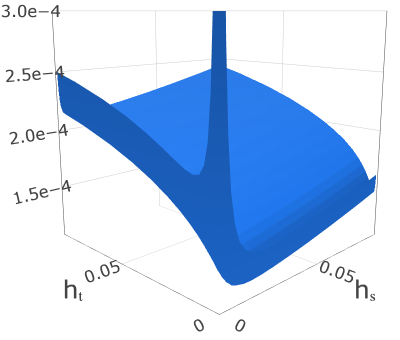
\includegraphics[width=0.35\textwidth]{./figures/autocov/plt_autocov_risk_conso_new_design_N=150_lambda=100_s=0.2_t=0.3.png} & 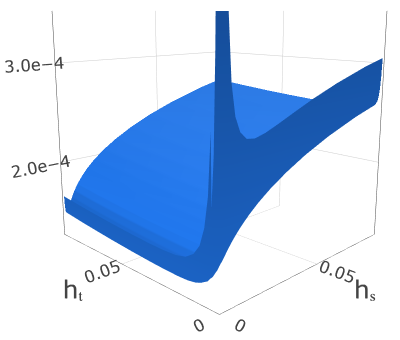
\includegraphics[width=0.35\textwidth]{./figures/autocov/plt_autocov_risk_conso_new_design_N=150_lambda=100_s=0.5_t=0.2.png}\\
		$(h_1^*(s|t), h_1^*(t|s)) = (0.001, 0.016)$ & $ (h_1^*(s|t), h_1^*(t|s)) = (0.021, 0.001)$ \\
		& \\
		& \\
		$(s, t)= (0.1, 0.4)$ & $(s, t)= (0.8, 0.5)$\\
		$(H_s, H_t)= (0.529, 0.527)$ & $(H_s, H_t)= (0.445, 0.784)$\\
		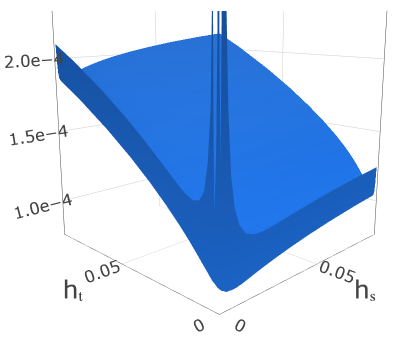
\includegraphics[width=0.35\textwidth]{./figures/autocov/plt_autocov_risk_conso_new_design_N=150_lambda=100_s=0.1_t=0.4.png} &
		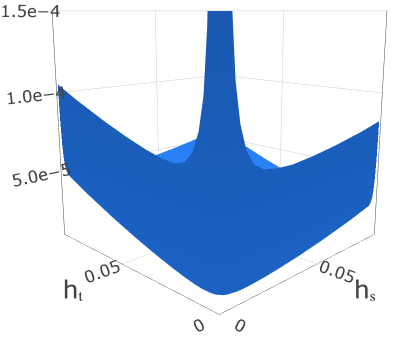
\includegraphics[width=0.35\textwidth]{./figures/autocov/plt_autocov_risk_conso_new_design_N=150_lambda=100_s=0.8_t=0.5.png}\\
		$(h_1^*(s|t), h_1^*(t|s)) = (0.003, 0.007)$ & $(h_1^*(s|t), h_1^*(t|s)) = (0.009, 0.012)$ 
	\end{tabular}
	\caption{\small Empirical average of the risk function $\widehat{R}_{\Gamma_1}(s,t;h_s, h_t)$ at $(s,t) \in \{ (0.2, 0.3)$, $(0.5, 0.2)$, $(0.1, 0.4)$, $(0.8, 0.5)\}$ computed over $400$ independent replications of the FTS for the sample size $(N, \lambda) = (150, 100)$. For each $(s,t)$, the optimal bandwidths $(h_1^*(s|t), h_1^*(t|s))$ corresponding to the plotted risk function are indicated at the bottom of the respective panel.}
	\label{fig:autocov_risk_2bw}
\end{figure}

We conclude this section with a performance comparison of the new autocovariance estimator against the \texttt{MPV24} estimator, which uses a single bandwidth. Let $\widehat{\Gamma}_{N,\ell}^{(i)}$ denote our new estimator computed from the $i$-th replication ($i = 1, \ldots, R = 400$), and let $\widehat{\Gamma}_{\texttt{MPV24}, \ell}^{(i)}$ denote the corresponding \texttt{MPV24} estimator. For benchmarking, we use the empirical infeasible estimator, denoted by ${\widehat{\Gamma}}_{N', \ell}$, which is computed on a large sample of size $N'$. This estimator is feasible in simulation settings. That is,
\begin{equation}
	\widehat{\Gamma}_{N', \ell}(s, t) = \frac{1}{N' - \ell} \sum_{n=1}^{N' - \ell} \left\{X_{n}(s) - \widehat{\mu}_{N'}(s)\right\} \left\{X_{n+\ell}(t) - \widehat{\mu}_{N'}(t)\right\},
	\qquad \text{where} \quad
	\widehat{\mu}_{N'}(t) = \frac{1}{N'} \sum_{n=1}^{N'} X_n(t).
\end{equation}
Then, for each $i = 1, \ldots, R$, we compute the pointwise error ratio:
\begin{equation}\label{eq:error_ratio_autocov}
	\forall (s, t) \in I^2, \quad
	E_\ell^{(i)}(s, t) = \frac{\left| \widehat{\Gamma}_{N,\ell}^{(i)}(s, t; h_\ell^*(s|t), h_\ell^*(t|s)) - \widehat{\Gamma}_{N',\ell}(s, t) \right|}{\left| \widehat{\Gamma}_{\texttt{MPV24}, \ell}^{(i)}(s, t; h^*) - \widehat{\Gamma}_{N',\ell}(s, t) \right|}.
\end{equation}
With $N' = 5000$, we compute the error ratios $\{E_1^{(i)}(s, t),\; i = 1, \ldots, R\}$ for the lag-1 autocovariance estimator at four locations $(s, t)$. Figure~\ref{fig:autocov_ratio_FTS_Conso} presents the corresponding boxplots across all $(N, \lambda)$ configurations. As anticipated from Theorem~\ref{thm:Gamma}, the new estimator significantly outperforms \texttt{MPV24} when the local regularities $H_s$ and $H_t$ differ, with greater gains observed for pairs $(s, t)$ such that $|H_s - H_t|$ is large. For instance, the largest improvements are found at $(s, t) = (0.2, 0.3)$ and $(0.5, 0.2)$, where $(H_{0.2}, H_{0.3}) = (0.199, 0.844)$ and $(H_{0.5}, H_{0.2}) = (0.784, 0.199)$, respectively. In contrast, at $(s, t) = (0.8, 0.5)$, where $(H_{0.8}, H_{0.5}) = (0.445, 0.784)$, the two estimators tend to perform similarly as the sample size increases.

\begin{figure}[h!]
	\centering
	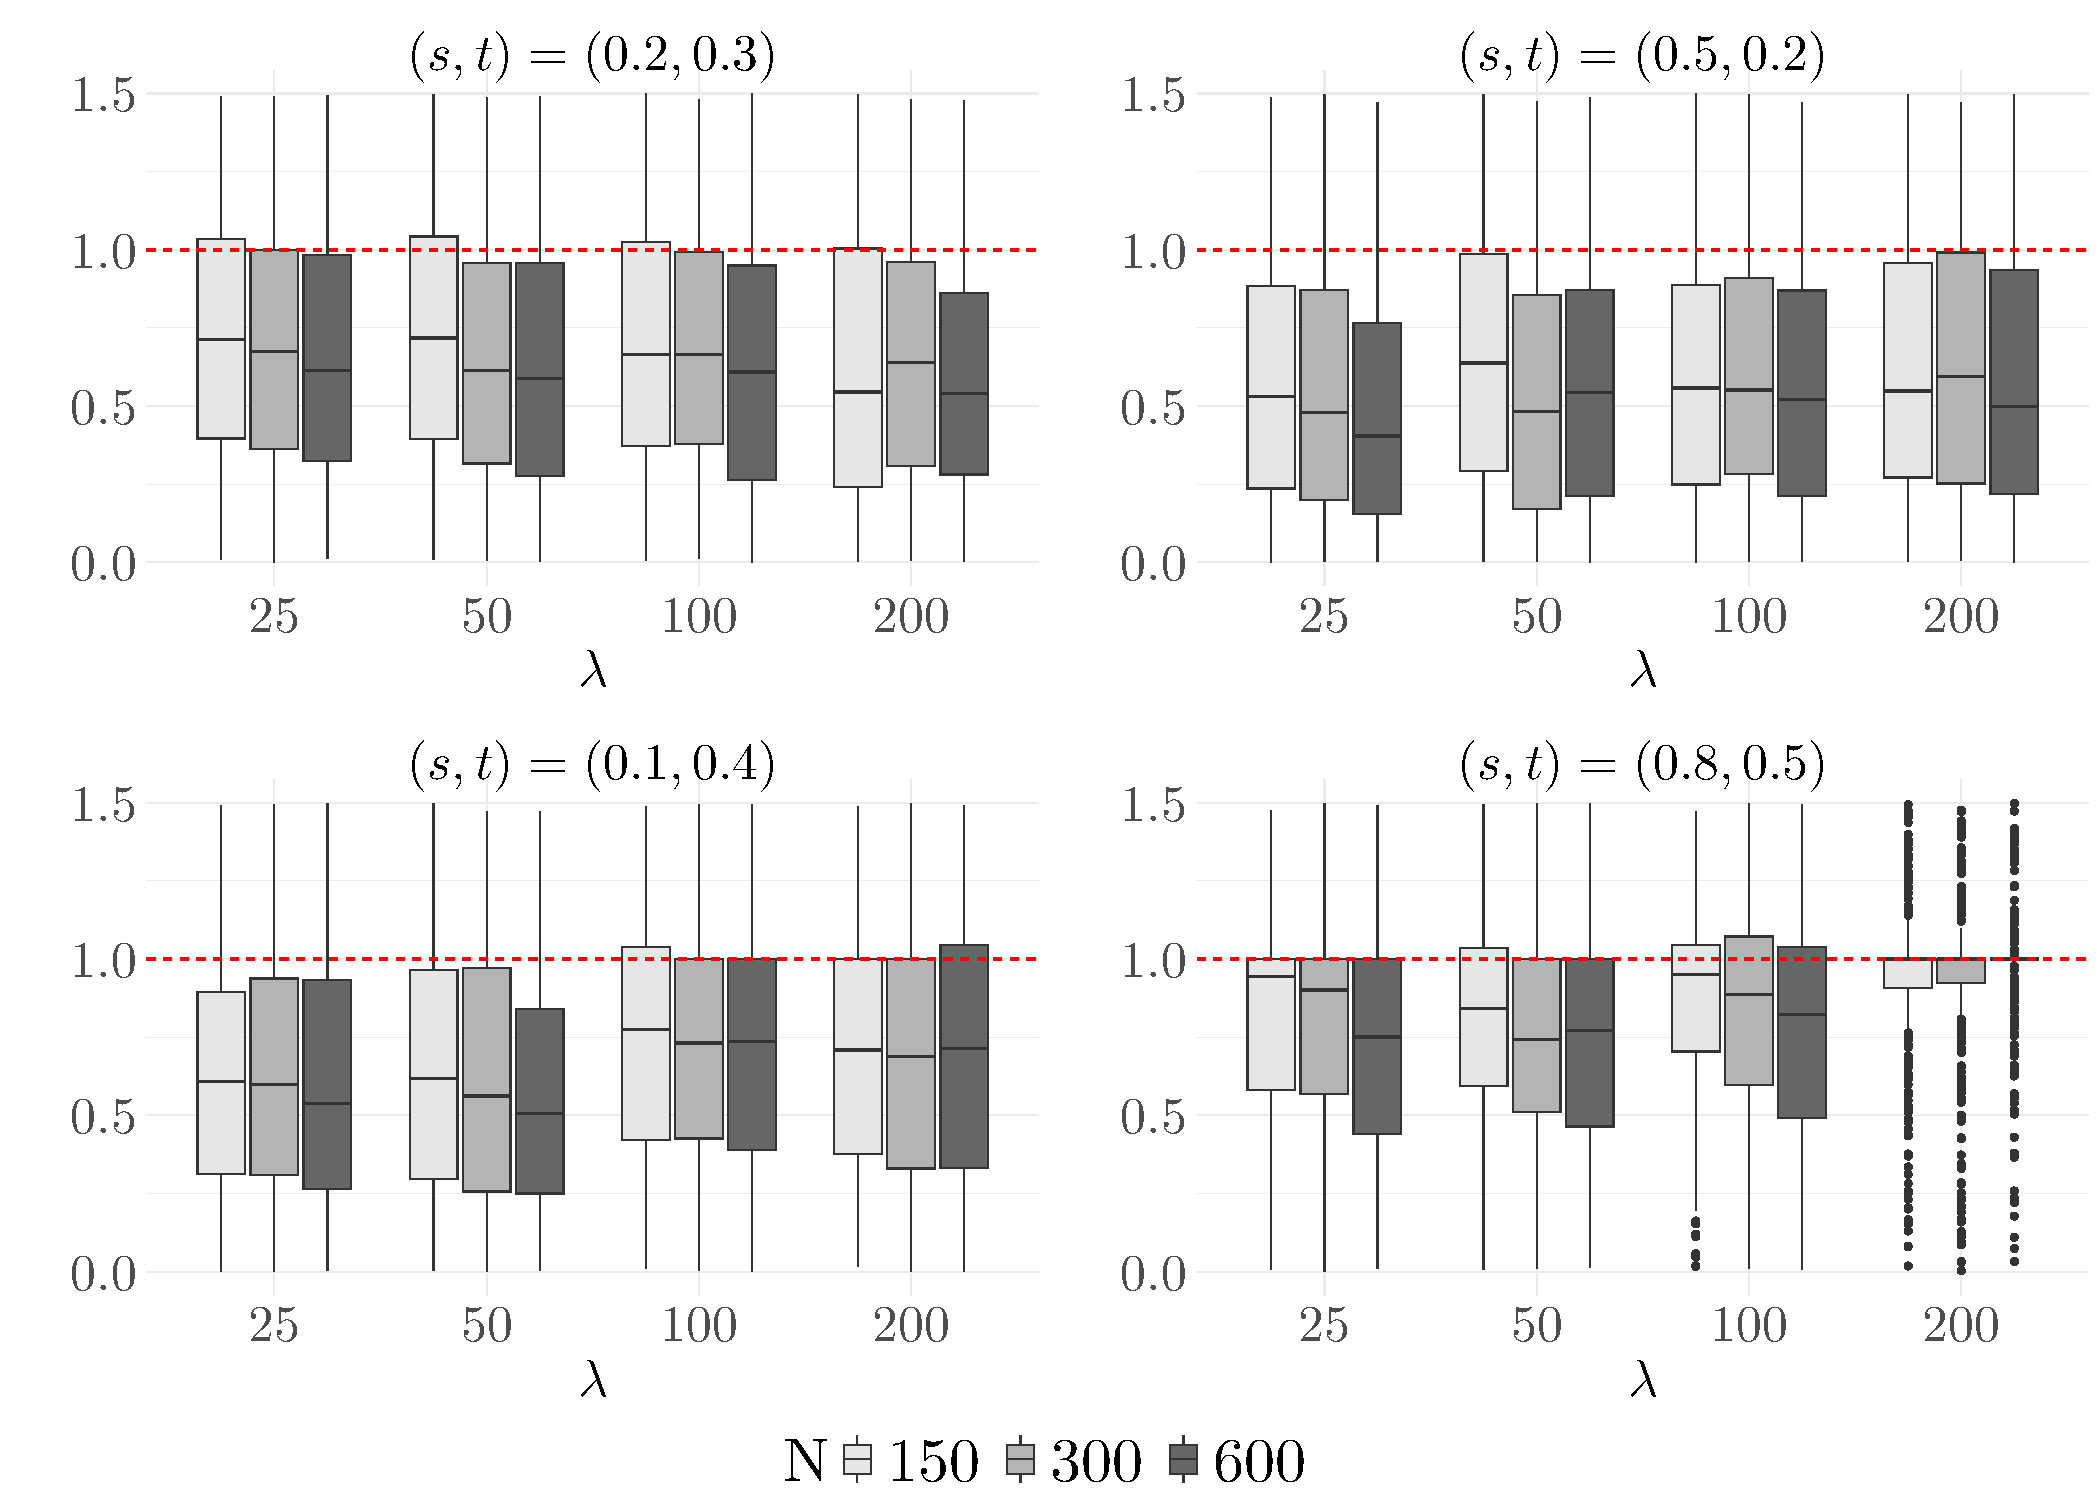
\includegraphics[width=0.9\textwidth]{./figures/autocov/boxplot_conso_autocov_ratio_new_design_lag=1_all_bis.pdf}
	\caption{\small Boxplots of the error ratio \eqref{eq:error_ratio_autocov} of the lag-1 autocovariance estimator for four pairs $(s, t) \in \{(0.2, 0.3)$, $(0.5, 0.2)$, $(0.1, 0.4)$, $(0.8, 0.5)\}$. For each pair, the corresponding values of the local exponent function are $(H_{0.2}, H_{0.3}) = (0.199, 0.844)$, $(H_{0.5}, H_{0.2}) = (0.784, 0.199)$, $(H_{0.1}, H_{0.4}) = (0.529, 0.527)$, and $(H_{0.8}, H_{0.5}) = (0.445, 0.784)$.}
	\label{fig:autocov_ratio_FTS_Conso}
\end{figure}

\subsection{Covariance function estimation}\label{sec:emp_study:cov}
Our new adaptive covariance estimator involves selecting optimal bandwidths by minimising both the estimates of the bivariate risk function \eqref{eq:risk-Gamma_0:diagonal_outside} outside the diagonal band and the estimates of the univariate risk function given in \eqref{eq:risk-Gamma_0} for the diagonal line estimator. We consider the same scenario and generated data as in the autocovariance estimation study to illustrate the performance of our new covariance estimator.  

First, regarding the risk function estimation, Figure~\ref{fig:cov_risk_2bw} shows the average over the $400$ replications of the estimates of the covariance risk function \eqref{eq:risk-Gamma_0:diagonal_outside} for $(N, \lambda) = (150, 100)$ at four locations. These plots provide evidence that the risk function is convex and can thus be effectively minimised to obtain optimal bandwidth pairs. Similarly, Figure~\ref{fig:diagonal_risk} illustrates that the risk function for the diagonal line is also convex, allowing straightforward selection of the optimal bandwidth for its estimation.

Furthermore, for the bivariate risk function \eqref{eq:risk-Gamma_0:diagonal_outside}, since the regularity varies across the domain (see Figure~\ref{fig:simu_param}-(a)), the optimal bandwidth pairs $(h_0^*(s|t), h_0^*(t|s))$ are typically such that $h_0^*(s|t) \neq h_0^*(t|s)$ when $H_s \neq H_t$. The difference between the selected bandwidths becomes more pronounced for pairs $(s, t)$ with large differences in local regularity, that is, when $|H_s - H_t|$ is large.

\begin{figure}[h!]
		\centering
	\begin{tabular}{cc}
		$(s, t)= (0.2, 0.3)$ & $(s, t)= (0.5, 0.2)$\\
		$(H_s, H_t)= (0.199, 0.844)$ & $(H_s, H_t)= (0.784, 0.199)$\\
		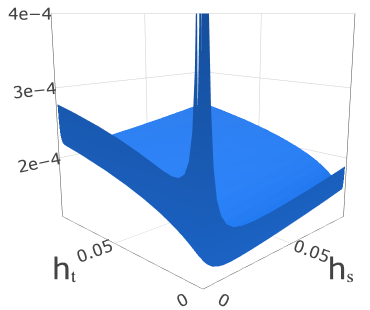
\includegraphics[width=0.35\textwidth]{./figures/cov/plt_cov_risk_conso_new_design_N=150_lambda=100_s=0.2_t=0.3.png} & 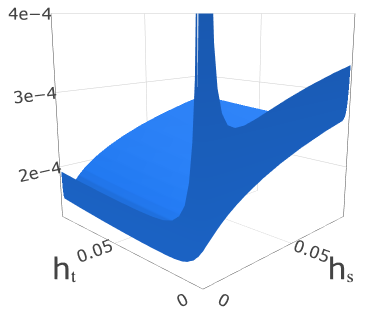
\includegraphics[width=0.35\textwidth]{./figures/cov/plt_cov_risk_conso_new_design_N=150_lambda=100_s=0.5_t=0.2.png}\\
		$(h_0^*(s|t), h_0^*(t|s)) = ( 0.002, 0.016)$ & $ (h_0^*(s|t), h_0^*(t|s)) = (0.021, 0.002)$ \\
		& \\
		& \\
		$(s, t)= (0.1, 0.4)$ & $(s, t)= (0.8, 0.5)$\\
		$(H_s, H_t)= (0.529, 0.527)$ & $(H_s, H_t)= (0.445, 0.784)$\\
		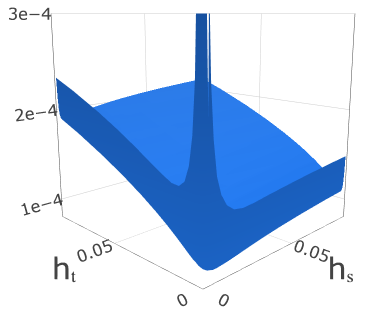
\includegraphics[width=0.35\textwidth]{./figures/cov/plt_cov_risk_conso_new_design_N=150_lambda=100_s=0.1_t=0.4.png} &
		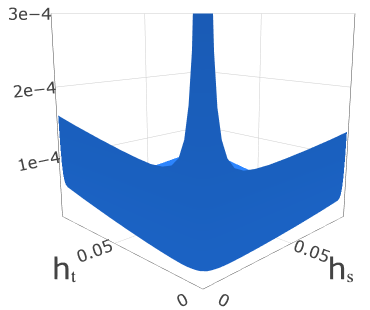
\includegraphics[width=0.35\textwidth]{./figures/cov/plt_cov_risk_conso_new_design_N=150_lambda=100_s=0.8_t=0.5.png}\\
		$(h_0^*(s|t), h_0^*(t|s)) = (0.003, 0.007)$ & $(h_0^*(s|t), h_0^*(t|s)) = (0.009, 0.016)$
	\end{tabular}
	\caption{\small Empirical average of the risk function $\widehat{R}_{\Gamma_0}(s,t;h_s, h_t)$ at $(s,t) \in \{ (0.2, 0.3)$, $(0.5, 0.2)$, $(0.1, 0.4)$, $(0.8, 0.5)\}$ computed over $400$ independent replications of the FTS for the sample size $(N, \lambda) = (150, 100)$. For each $(s,t)$, the optimal bandwidths $(h_0^*(s|t), h_0^*(t|s))$ corresponding to the plotted risk function are indicated at the bottom of the respective panel.}
	\label{fig:cov_risk_2bw}
\end{figure}
\begin{figure}[th]
	\vspace{.1cm}
	\centering
	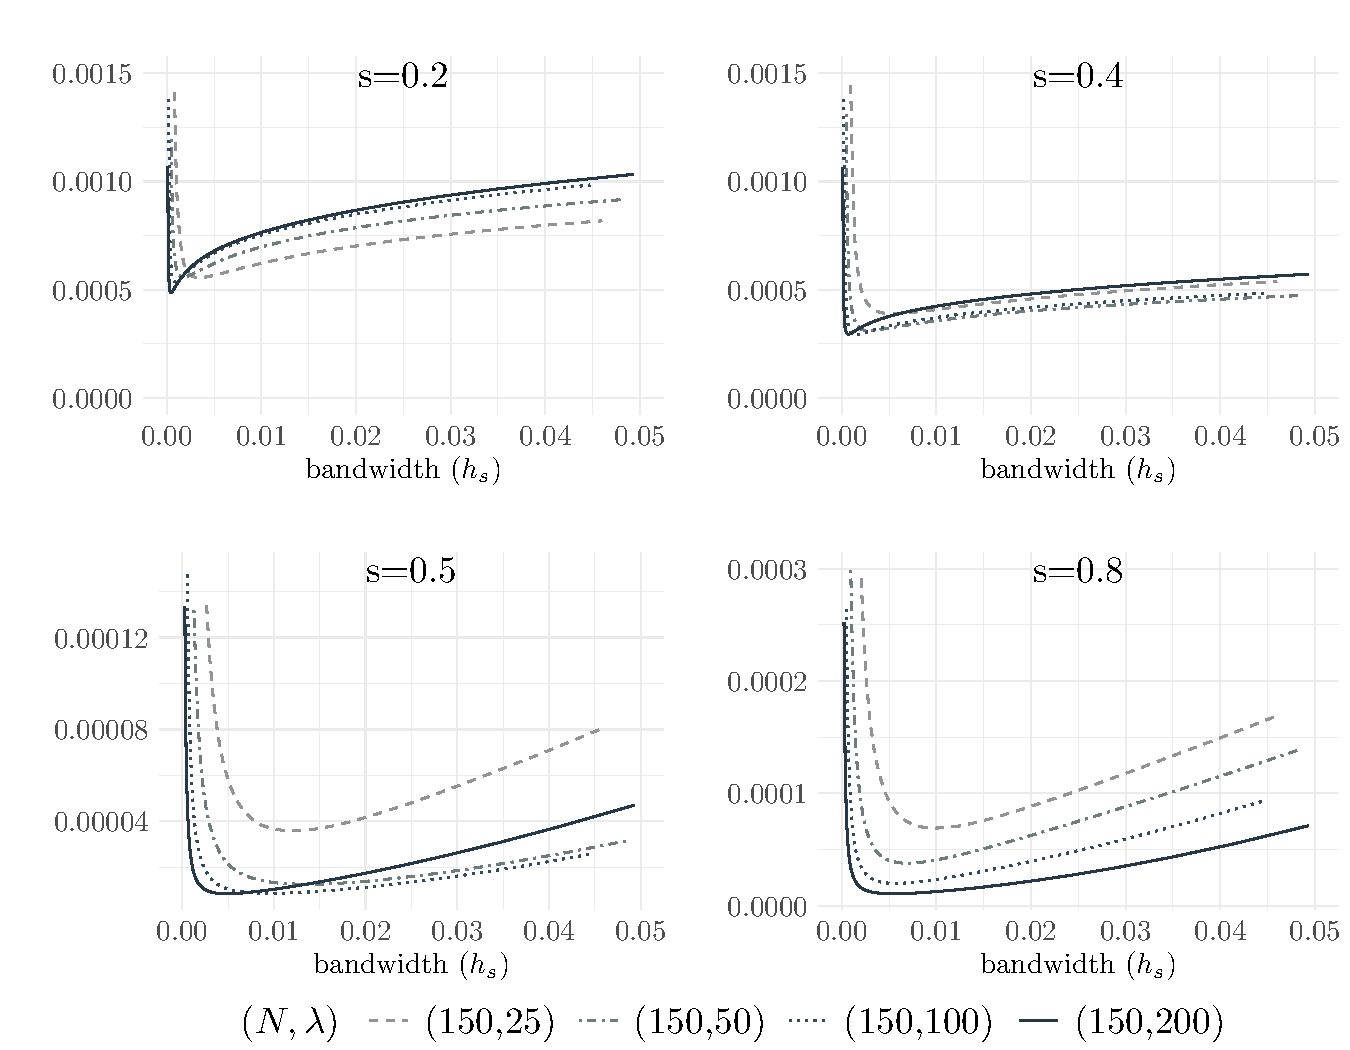
\includegraphics[width=0.9\linewidth]{./figures/cov/plt_diag_cov_risk_conso_new_design_N=150_all_lambda_all_s.pdf}
	\caption{\small Empirical average of the risk function $\widehat{R}_\mu(s, h_s)$ at $s \in \{0.2, 0.4, 0.5, 0.8\}$, computed over $400$ independent replications of the FTS for sample sizes $(N, \lambda) \in \{(150, 25), (150, 50), (150, 100), (150, 200)\}$.}
	\label{fig:diagonal_risk}
\end{figure}

We conclude this section with a performance comparison between our proposed covariance estimator and its version that selects the same bandwidth for both arguments of the function. The error in \eqref{eq:error_ratio_autocov} is then computed with respect to that covariance estimator instead of to the \texttt{MPV24} estimator. For simplicity, we do not restate the formula. Figure~\ref{fig:cov_ratio_FTS_Conso} shows boxplots of the error ratio of the covariance estimator for four $(s, t)$ pairs across different sample size configurations $(N, \lambda)$. As anticipated from Theorem~\ref{thm:Gamma_0}, our estimator significantly outperforms the covariance estimator that uses the same local optimal bandwidth for both arguments, when the local regularities $H_s$ and $H_t$ differ, and the gain increases with larger values of $|H_s - H_t|$.

\begin{figure}[h!]
	\centering
	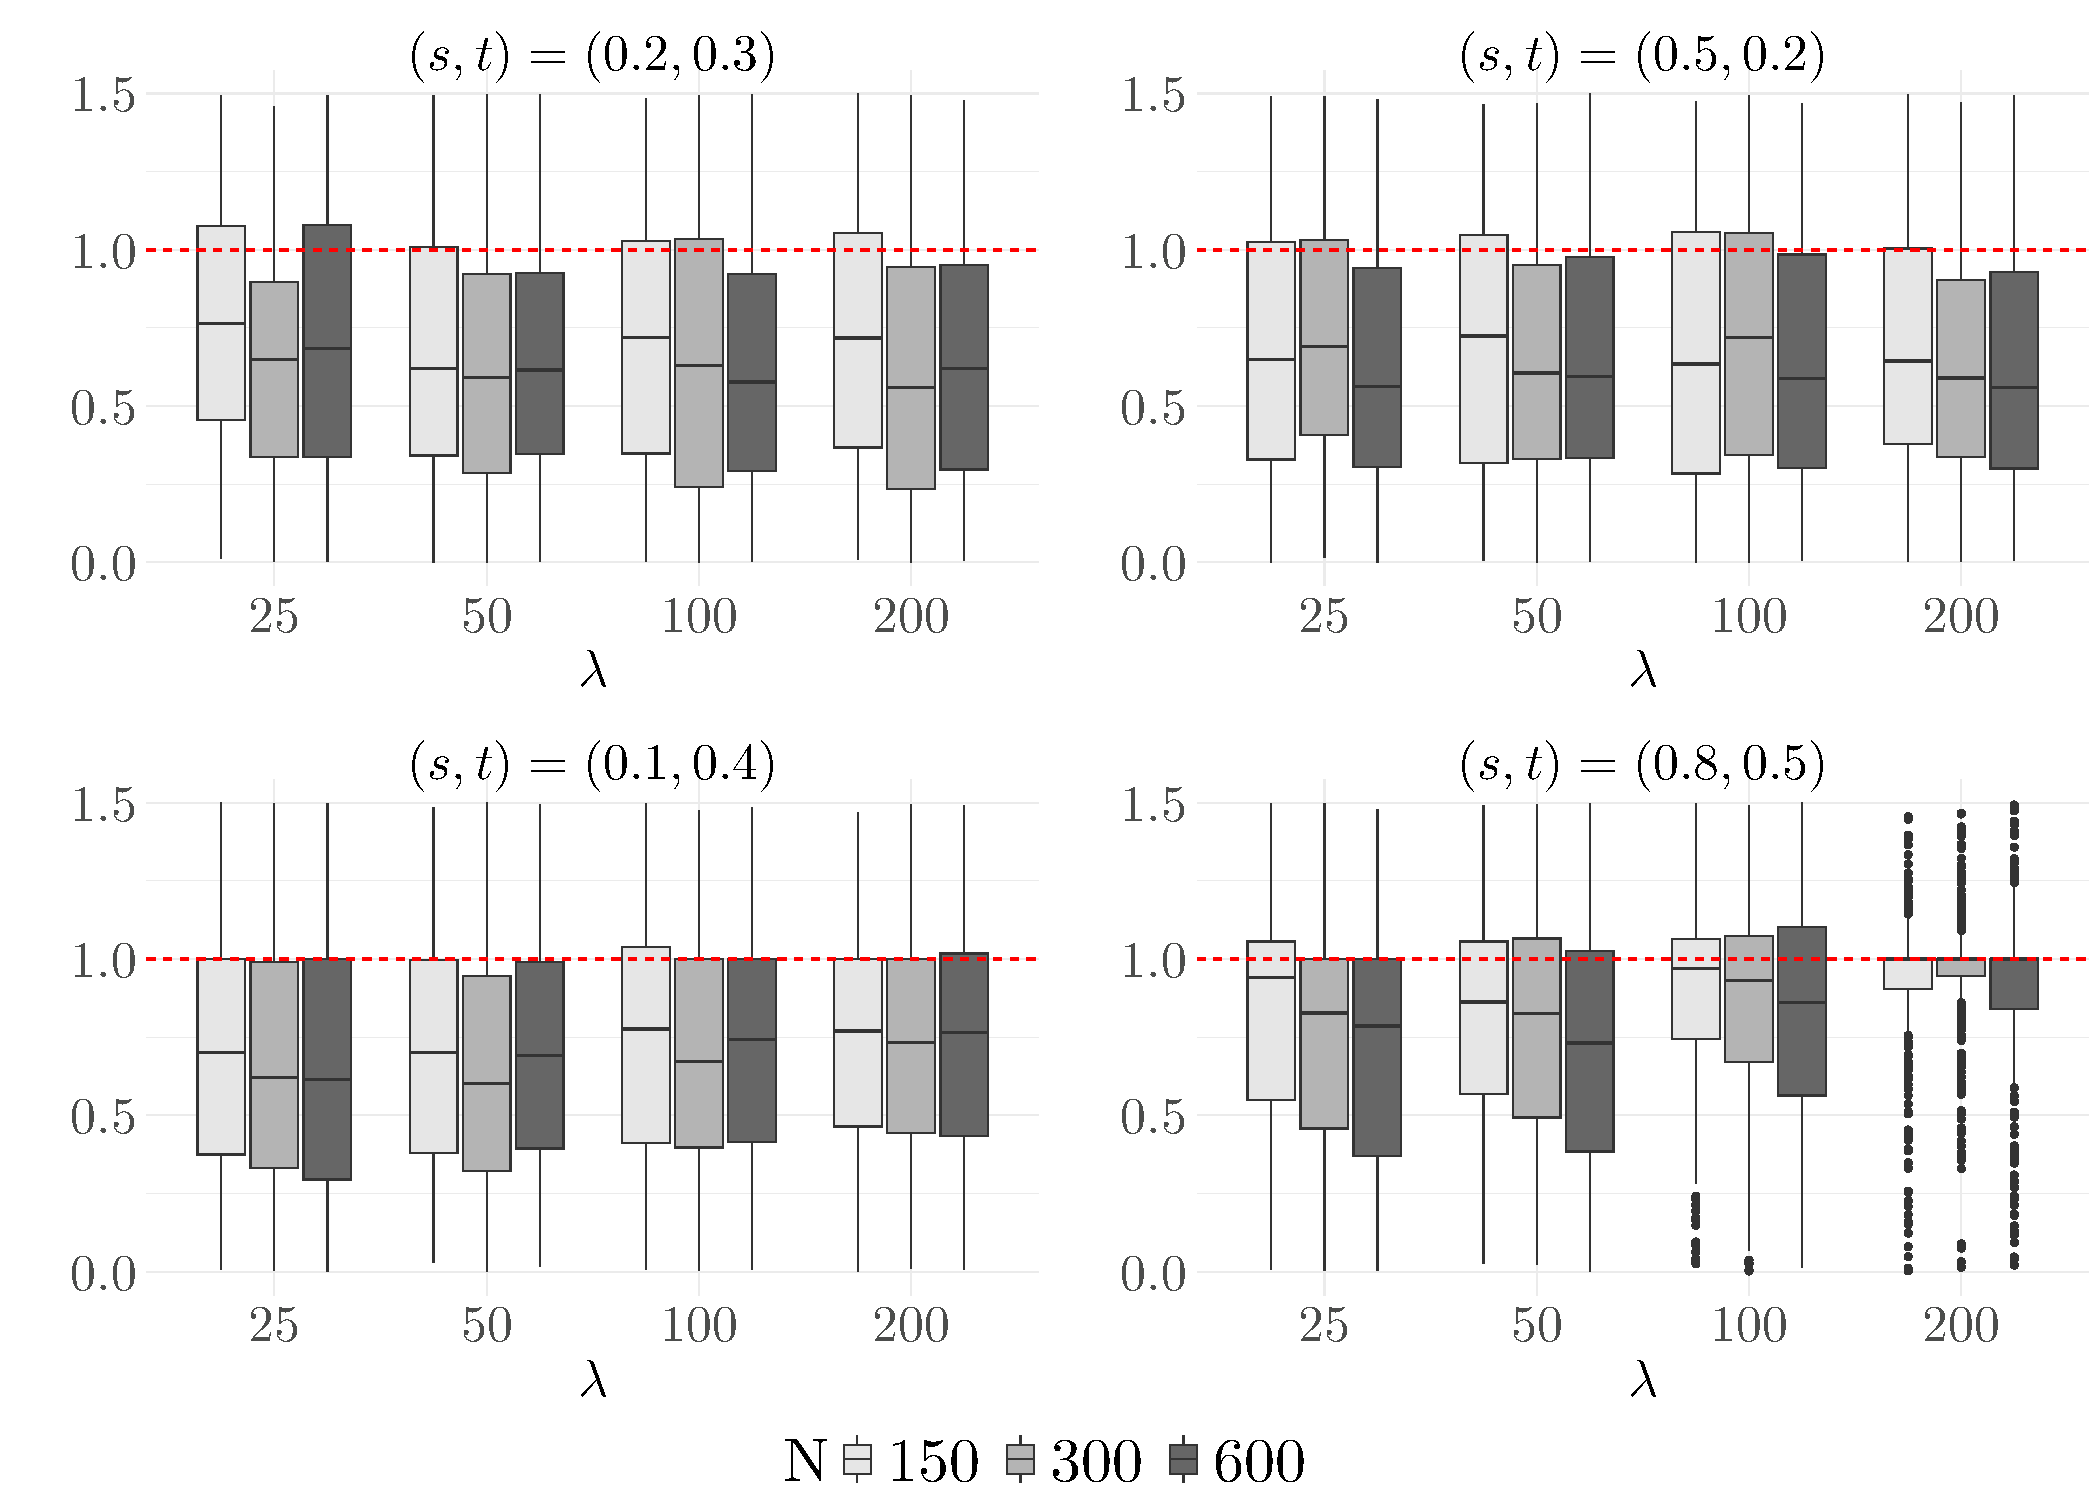
\includegraphics[width=0.9\textwidth]{./figures/cov/boxplot_conso_cov_ratio_new_desing_lag=0_all_bis.pdf}
	\caption{\small Boxplot of the error ratio \eqref{eq:error_ratio_autocov} of the covariance estimator for four pairs $(s, t) \in \{(0.2, 0.3)$, $(0.5, 0.2)$, $(0.1, 0.4)$, $(0.8, 0.5)\}$. For each pair, the corresponding values of the local exponent function are $(H_{0.2}, H_{0.3}) = (0.199, 0.844)$, $(H_{0.5}, H_{0.2}) = (0.784, 0.199)$, $(H_{0.1}, H_{0.4}) = (0.529, 0.527)$, and $(H_{0.8}, H_{0.5}) = (0.445, 0.784)$.} 
	\label{fig:cov_ratio_FTS_Conso}
\end{figure}

\subsection{Adaptive curve prediction}
In this section, we study the performance of the adaptive BLUP through Monte Carlo simulations. Since the adaptive BLUP leverages information from both the current curve and the lagged curve, we first examine the empirical autoregressive effect and then present the Monte Carlo results.

\subsubsection{Empirical autoregressive effect}

Recall that the adaptive BLUP depends on adaptive estimates of the mean, covariance, and lag-$1$ autocovariance functions. To describe the strength of dependence between the current and lagged curves, we compute a functional analogue of the autocorrelation function for real-valued time series. The Functional Autocorrelation Function (FACF) at lag~$\ell$, considered by \citet{horovath_2016}, is defined as
\begin{equation}\label{eq:blup:facf}
	\widehat{\rho}_\ell = 
	\|\widehat{\Gamma}_{N,\ell}\|\left[\int \widehat{\Gamma}_{N,0}(t,t)dt\right]^{-1},
\end{equation}
where $\widehat{\Gamma}_{N,\ell}$ estimates $\Gamma_\ell$, and $\|\cdot\|$ denotes the standard norm in $\mathbb{L}^2_\mathcal{H}$. Moreover, $0 \leq \widehat{\rho}_\ell \leq 1$. The FACF also serves as an empirical check for the presence of an autoregressive effect in the FTS. In fact, if there were no autoregressive effect, the FACF would equal zero, implying that the autocovariance-related top-right and bottom-left blocks in the matrix $\VV_{n_0}$ would be nil and thus contribute nothing to the adaptive BLUP.

\begin{figure}[h]
	\centering
	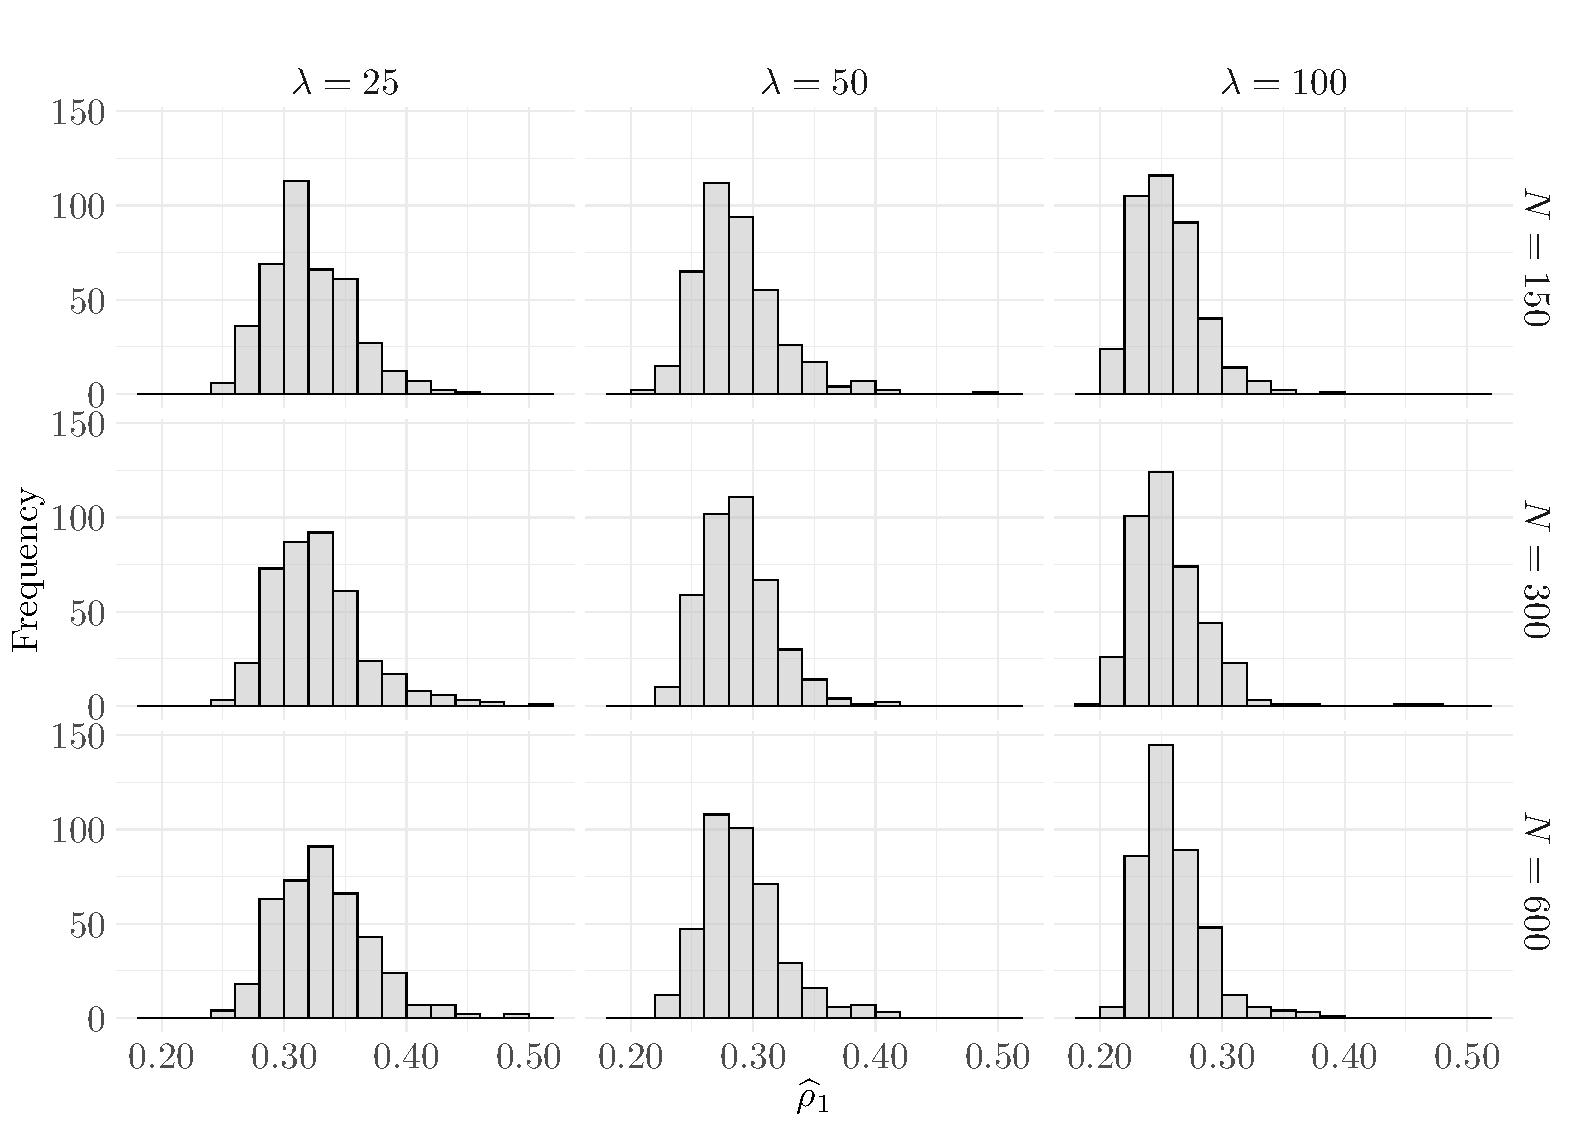
\includegraphics[width=\textwidth]{./figures/blup/hist_lag-1_facf_conso.pdf}
	\caption{\small Histograms of estimated lag-$1$ FACF values for different $(N, \lambda)$ configurations.}
	\label{fig:conso_lag1_facf}
\end{figure}

We use the same generated sample of FTS as in the study of the autocovariance function, estimate the lag-$1$ FACF for each of the $400$ FTS replications using \eqref{eq:blup:facf}, and display the resulting histograms in Figure~\ref{fig:conso_lag1_facf} for different sample sizes $(N, \lambda)$. The plots provide empirical evidence that the autocovariance-related blocks in $\VV_{n_0}$ are not nil. Moreover, for our simulated FAR(1) model, most of the lag-$1$ FACF values are concentrated between $0.2$ and $0.4$.

\subsubsection{Monte Carlo study}

We now turn to the study of the predictive performance of the adaptive BLUP through Monte Carlo simulations. Given a sample of FTS, the objective is to assess the prediction performance of its final curve, that is, $n_0 = N$, under various scenarios depending on the available observation points for that curve. To this end, we adopt a simulation setup that differs slightly from the one used in the study of the (auto)covariance function. 
We consider the pairs $(N, \lambda) \in \{150, 300, 600\} \times \{25, 50, 100\}$, generate a single sample of FTS, and regenerate its final curve $R = 400$ times.
The prediction accuracy of each regenerated final curve is then evaluated, given all or only a subset of its observed points, while maintaining the other curves of the FTS sample unchanged.

Table~\ref{tab:blup_fts_conso} shows the bias and standard deviation of the estimates of $\widehat{\mathfrak{X}}_{n_0}(t)$ obtained for the prediction of the last curve, when all observation points $\{(Y_{n_0, i}, T_{n_0,i}),\; 1\leq i \leq M_{n_0}\}$ are available. As expected, both the bias and the variance of the adaptive BLUP decrease as the sample size increases. Notably, the estimated standard deviation tends to increase with $t$. This is partly due to the sample paths becoming rougher towards the right end of the domain $I$, as illustrated by the shape of the local exponent function in Figure~\ref{fig:simu_param}-(a). Moreover, larger values of $t$ are associated with higher marginal variance $\operatorname{Var}(X_t)$, as shown in Figure~\ref{fig:var_FTSConso}. These factors lead to less accurate estimates of the mean and (auto)covariance functions, and consequently to less accurate predictions by the adaptive BLUP.

\begin{table}[!tbp]
	\begin{center}
		{\small 	
			\begin{tabular}{cccccccccccccc}
				\hline
				&&&\multicolumn{2}{c}{\bfseries $t = 0.2$}&&\multicolumn{2}{c}{\bfseries $t = 0.4$}&&\multicolumn{2}{c}{\bfseries $t = 0.7$}&&\multicolumn{2}{c}{\bfseries $t = 0.8$}\\
				\cline{4-5} \cline{7-8} \cline{10-11} \cline{13-14}
				\multicolumn{1}{c}{$N$}&\multicolumn{1}{c}{$\lambda$}&&\multicolumn{1}{c}{Bias}&\multicolumn{1}{c}{Sd}&&\multicolumn{1}{c}{Bias}&\multicolumn{1}{c}{Sd}&&\multicolumn{1}{c}{Bias}&\multicolumn{1}{c}{Sd}&&\multicolumn{1}{c}{Bias}&\multicolumn{1}{c}{Sd}\tabularnewline
				\hline
				$150$&$ 25$&&0.0229&0.1173&&-0.0187&0.1209&&0.0331&0.1404&&0.0001&0.1275\\
				$150$&$ 50$&&0.0430&0.1033&&0.1017&0.1293&&-0.0050&0.1194&&-0.0093&0.1285\\
				$150$&$100$&&-0.0085&0.1006&&0.0672&0.0994&&0.0232&0.1326&&-0.0207&0.1005\\
%				$300$&$ 25$&&0.0076&0.0885&&-0.0272&0.1052&&-0.0367&0.1036&&0.0078&0.1315\\
%				$300$&$ 50$&&0.0247&0.1392&&0.0482&0.1316&&0.0305&0.1376&&-0.0505&0.1403\\
%				$300$&$100$&&0.0192&0.1018&&0.0076&0.1291&&0.0235&0.1223&&-0.0638&0.1221\\
%				$600$&$ 25$&&0.0097&0.0932&&0.0044&0.1114&&-0.014&0.1418&&0.0019&0.1292\\
%				$600$&$ 50$&&-0.0030&0.1047&&0.0656&0.1055&&0.0457&0.1344&&-0.0243&0.1245\\
%				$600$&$100$&&-0.0437&0.1052&&0.0102&0.1222&&0.0190&0.1408&&0.0773&0.1238\\
				\hline
		\end{tabular} }
		\caption{\small Bias and standard deviation (SD) of adaptive BLUP estimates for the last curve, based on $400$ independent replications.}
		\label{tab:blup_fts_conso}
	\end{center}
\end{table}

We now compare our prediction procedure to that of \citet{rubin2020sparsely}, referred to as \texttt{RP20}, as well as to the Nadaraya–Watson (NW) estimator using a cross-validated bandwidth as defined in \eqref{eq:NW_bw_cv}. The comparison with the NW estimator is limited to the scenario where all observation points on the last curve are available. For the comparison with \texttt{RP20}, we also consider three additional scenarios in which the available observation points for the last curve lie within the subdomains $(0, 1/4]$, $(0, 1/2]$, and $(0, 3/4]$.

\begin{figure}[ht!]
	\centering
	\begin{tabular}{c}
		ISE ratio w.r.t. \texttt{NW} estimator\\
		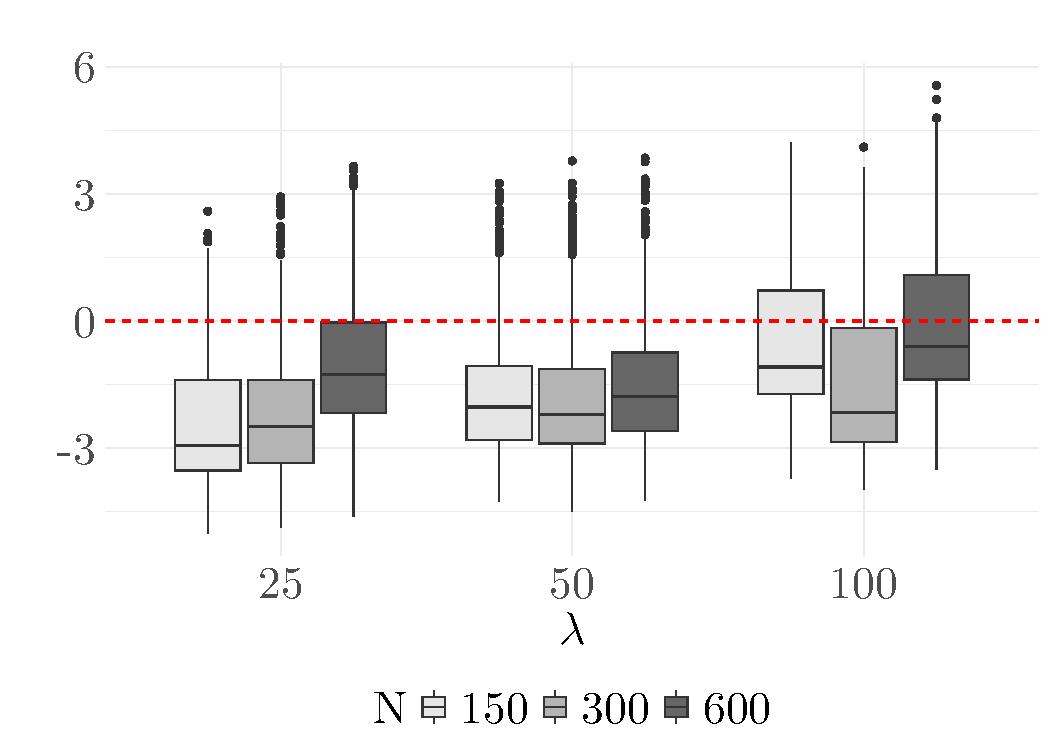
\includegraphics[width=0.5\textwidth]{./figures/blup/plot_log_ise_ratio_blup_2bw_over_nw.pdf}
	\end{tabular}
	\caption{\small Boxplots of the $\log$ ISE ratios of the adaptive BLUP relative to the NW estimator, in the scenario where all observation points of the last curve to be predicted are available.}
	\label{fig:ise_ratio_blup_nw}
\end{figure}

Let us denote by
\begin{equation}
	\mathcal{T}_{n_0}^\alpha = \{ (Y_{n,i}, T_{n, i}) \; : \; T_{N, i} \in (0, \alpha], \; 1 \leq i \leq M_{n}, \; 1 \leq n \leq N\}, \qquad \alpha=1/4, 1/2, 3/4,
\end{equation}
the set of all available observation points in the FTS, with the last curve observed only over $(0, \alpha]$. Predictions based on the data $\mathcal{T}_{n_0}^\alpha$ are compared using the ratio of integrated squared errors (ISE). Let the superscript $(k)$ denote the $k$-th replication of the last curve. Then, the ISE ratio of the adaptive BLUP relative to a given method $\texttt{Meth}$ (either NW or \texttt{RP20}) is defined as
\begin{equation}
	\text{Ratio}^{(k)}(\texttt{Meth}) = \dfrac{\int_0^1 \left(\widehat{\mathfrak{X}}_{n_0}^{(k)}(t) - X_{n_0}^{(k)}(t)\right)^2 dt}{ \int_0^1 \left(\widehat{\mathfrak{X}}_{\texttt{Meth}}^{(k)}(t) - X_{n_0}^{(k)}(t)\right)^2 dt}.
\end{equation}

\begin{figure}[h!]
	\centering
	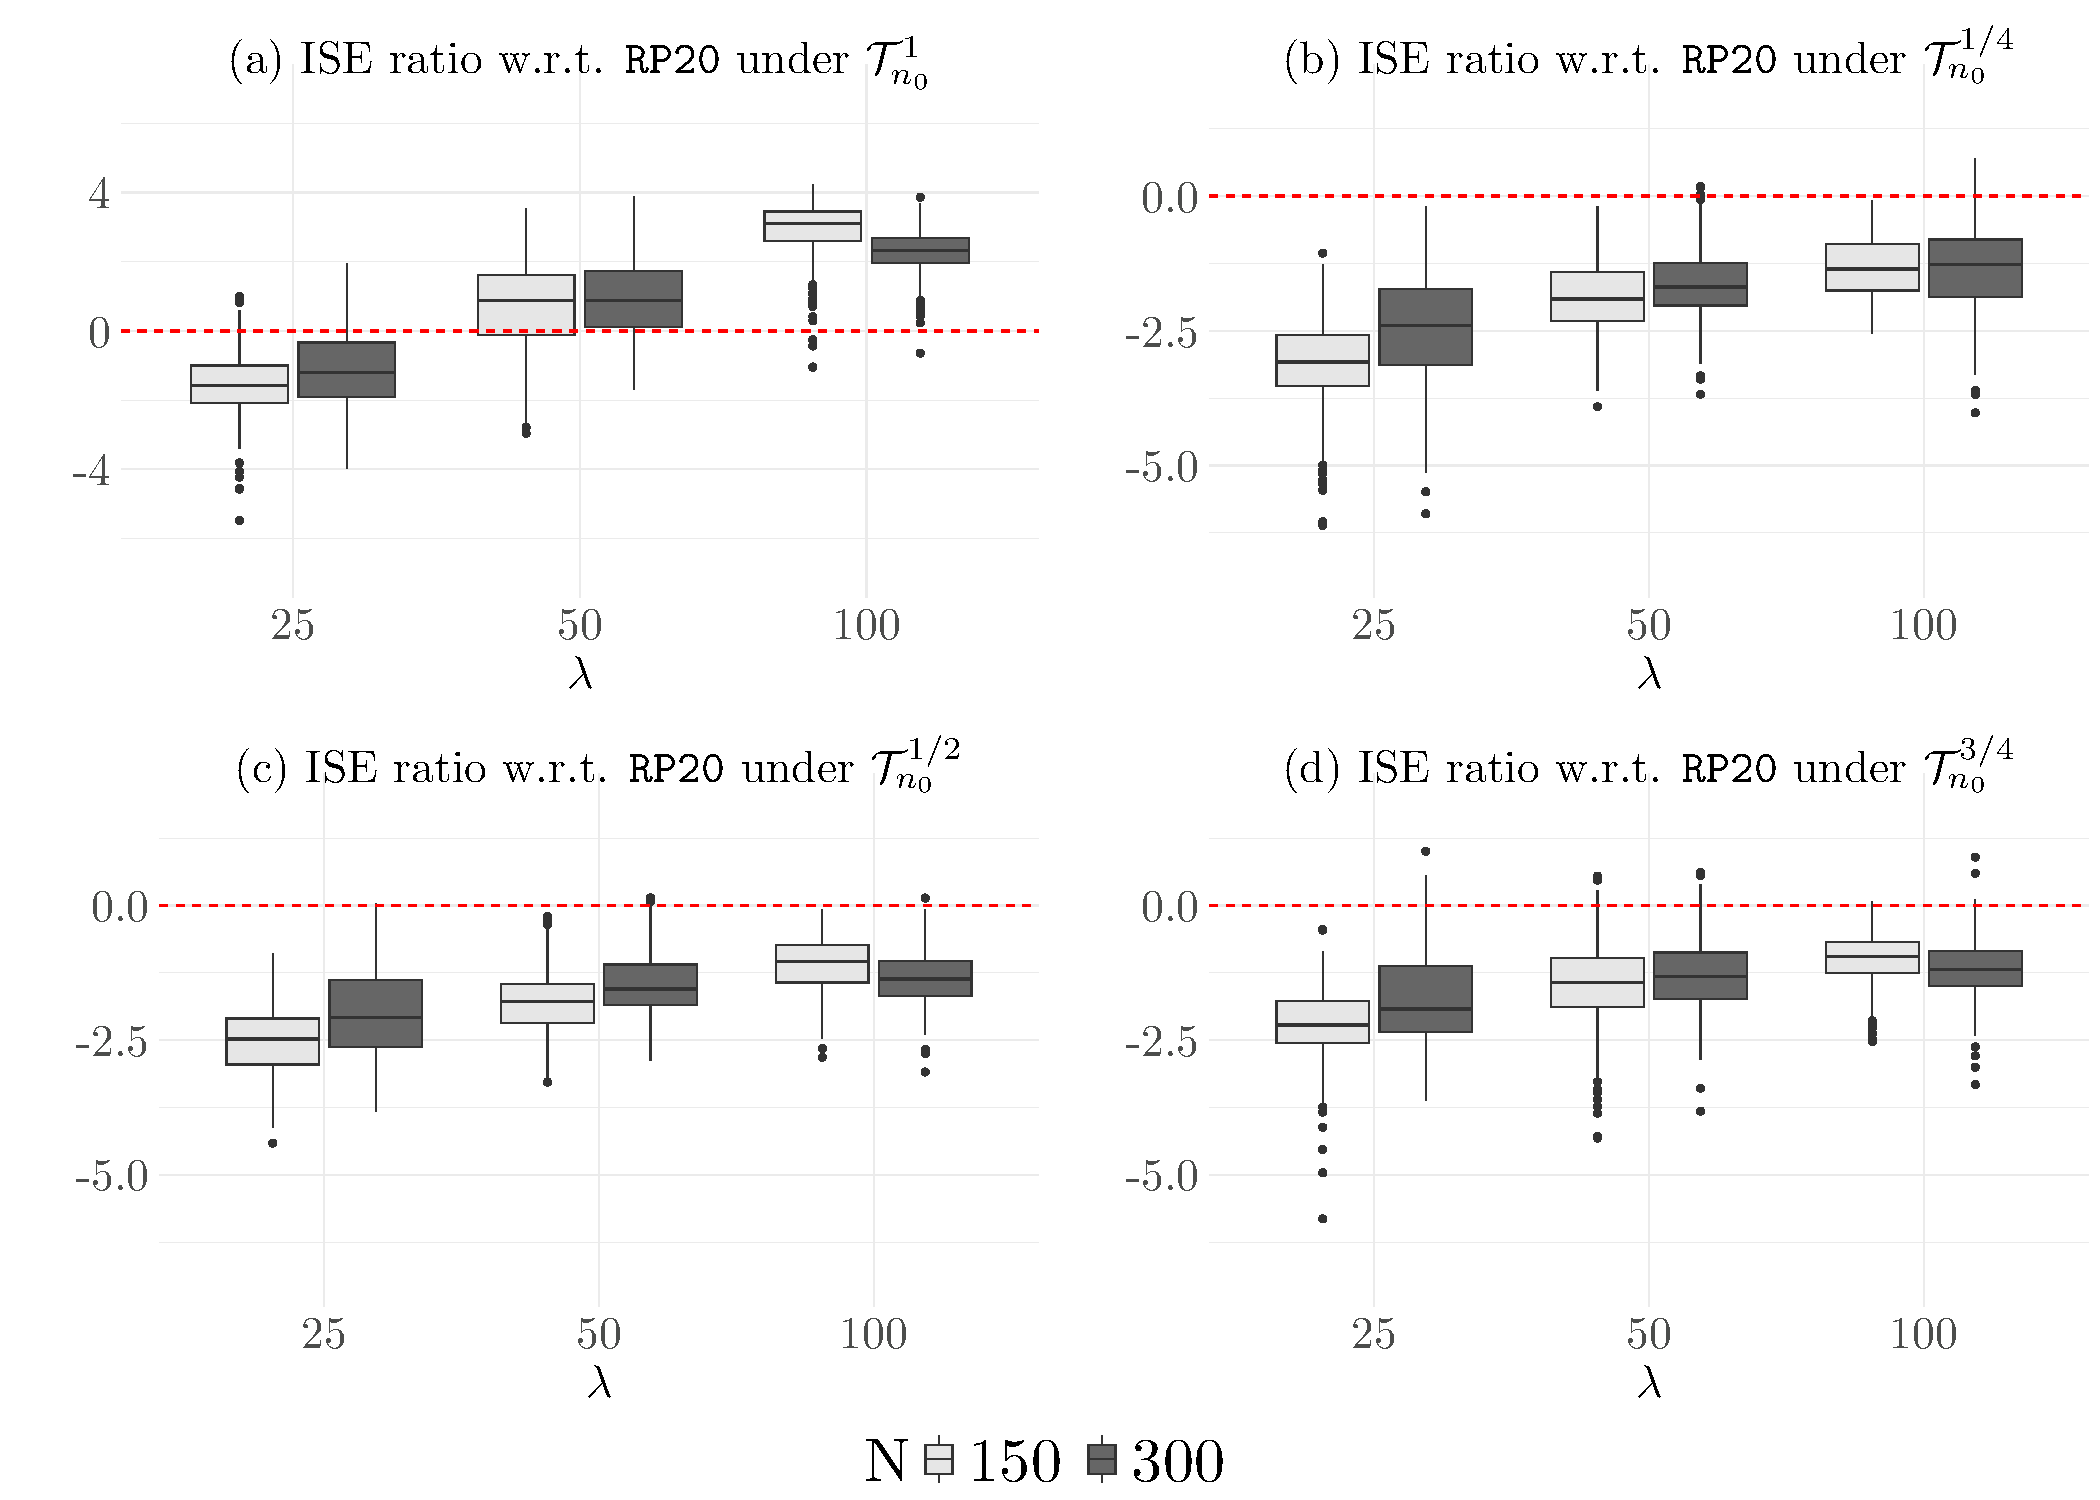
\includegraphics[width=0.9\textwidth]{./figures/blup/log_ise_ratio_blup_over_RP20_new_design_all.pdf}
	\caption{\small Boxplots of the $\log$ ISE ratios of the adaptive BLUP relative to \texttt{RP20} for predicting the last curve, with available observations in $(0, 1]$, $(0, 1/4]$, $(0, 1/2]$, and $(0, 3/4]$, respectively.}
	\label{fig:ise_ratio_blup_rp}
\end{figure}

Recall that the \texttt{RP20} method is a BLUP-based approach, where the mean is estimated using a local linear smoother and the lag-$\ell$ (auto)covariance function is estimated using a local linear surface smoother (off-diagonal, when $\ell = 0$) and a local quadratic smoother (on the diagonal, when $\ell = 0$). Smoothing bandwidths are selected via $K$-fold cross-validation coupled with Bayesian optimisation (implemented in MATLAB). Observations are randomly sampled on a regular grid of 241 points, and B-spline projections are used to reduce the computational time during optimisation.

Figure~\ref{fig:ise_ratio_blup_nw} presents boxplots of the logarithm of the ISE ratios of the adaptive BLUP relative to the NW estimator. These plots show that the adaptive BLUP generally outperforms the NW estimator, with the $\log$-relative gain tending to zero as $\lambda$ increases. When $\lambda \in \{25, 50\}$, the adaptive BLUP clearly provides better performance. However, for $\lambda = 100$, the NW estimator becomes more accurate and tends to perform similarly to the adaptive BLUP. This is likely due to the decrease in the mean squared error of the NW estimator as $\lambda$ increases, which improves its ability to reconstruct the curves effectively.

Figure~\ref{fig:ise_ratio_blup_rp} shows the boxplots of the $\log$ ISE ratios of the adaptive BLUP relative to the \texttt{RP20} method under the four scenarios $\alpha = 1, 1/4, 1/2$, and $3/4$. In the full-observation case ($\alpha = 1$), the adaptive BLUP outperforms \texttt{RP20} when $\lambda = 25$, although this advantage diminishes as $N$ increases. However, for $\lambda \in \{50, 100\}$, \texttt{RP20} yields better performance than the adaptive BLUP (see Figure~\ref{fig:ise_ratio_blup_rp}-(a)). In contrast, in the partial-observation scenarios with $\alpha \in \{1/4, 1/2, 3/4\}$, the adaptive BLUP consistently outperforms \texttt{RP20} across all considered combinations of $(N, \lambda)$, as illustrated in Figures~\ref{fig:ise_ratio_blup_rp}-(b), (c), and (d), respectively.


%\FloatBarrier

\subsection{Real data application}
We consider the prediction of daily Facebook stock volume curves. The dataset, available at \url{https://firstratedata.com/}, contains one-minute time-frame records of the stock price and volume. We extract observations from 1 January 2021 to 31 March 2022, using only the market’s regular trading hours, from 9:30~a.m to 4:00~p.m.

We construct daily stock return curves as the difference between the logarithm of the price at each time during the day and the opening price at 9:30~a.m. We are interested in predicting the traded volume when the absolute value of the return exceeds 0.5\%. Thus, for each day, we retain only the stock volume observations where the absolute return is greater than 0.5\%. The resulting daily volume curves are observed at random times between 9:30~a.m. and 4:00~p.m., with a maximum of 390 points per curve, corresponding to the total number of minutes during regular trading hours. The observation times are normalised to the interval $(0,1]$. It is worth noting that traded volume is typically very high near the market’s close; to mitigate the impact of extreme values, we exclude any volume observations above the 97.5th percentile of the entire sample.

Figure~\ref{fig:facebook_volume_last_curves} shows the last four curves in the time series. Note that, due to the return threshold, a curve may have no observations satisfying the condition on a given day. Such cases account for fewer than 10\% of all days and, therefore, we neglect the effect of this missingness. The final dataset consists of 284 curves with an average of 282 points per curve.

\begin{figure}[h]
	\centering
	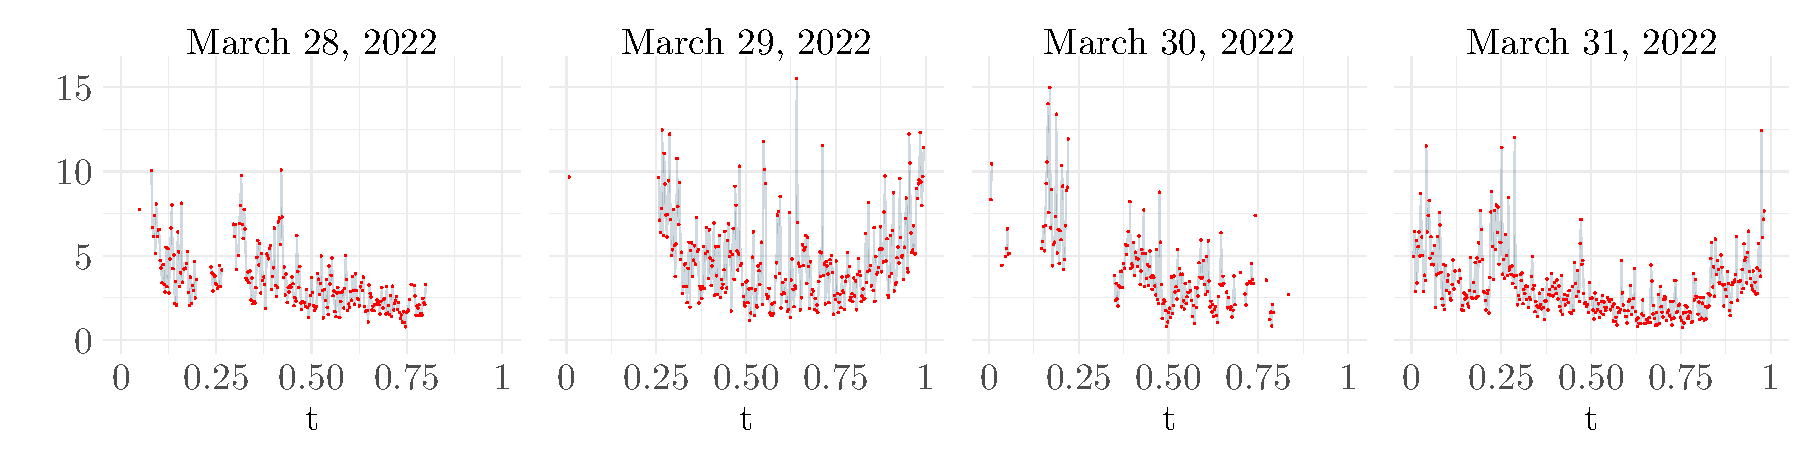
\includegraphics[width=\textwidth]{./figures/blup/Facebook_volume_4last_curves.pdf}
	\caption{\small Observation points for the last four daily Facebook stock volume curves in the dataset, with values normalised by $10^4$. Dots indicate the observation points, while the shaded lines illustrate the pattern between them.}   
	\label{fig:facebook_volume_last_curves}
\end{figure}

To assess the empirical autoregressive structure, we estimate the lag-$1$ FACF using \eqref{eq:blup:facf}, obtaining a value of $0.31$. This provides evidence that the autocovariance-related blocks in $\VV_{n_0}$ are non-negligible, indicating that the lagged curve contributes meaningfully to the adaptive BLUP. Moreover, this estimated FACF falls within the empirical distribution of lag-$1$ FACF values observed in our simulation study (see Figure~\ref{fig:conso_lag1_facf}).
 
Figure~\ref{fig:facebook_real_data_blup} presents a comparison between the adaptive BLUP predictions and the true stock volume curve to be predicted, together with a 95\% pointwise confidence interval. The comparison is performed under three scenarios, in which the available observations for the curve to be predicted are restricted to the interval $(0, \alpha]$ with $\alpha \in \{1/4, 1/2, 3/4\}$. Across these scenarios, the adaptive BLUP effectively captures local irregularities and demonstrates satisfactory predictive performance.

\begin{figure}[h]
	\centering
	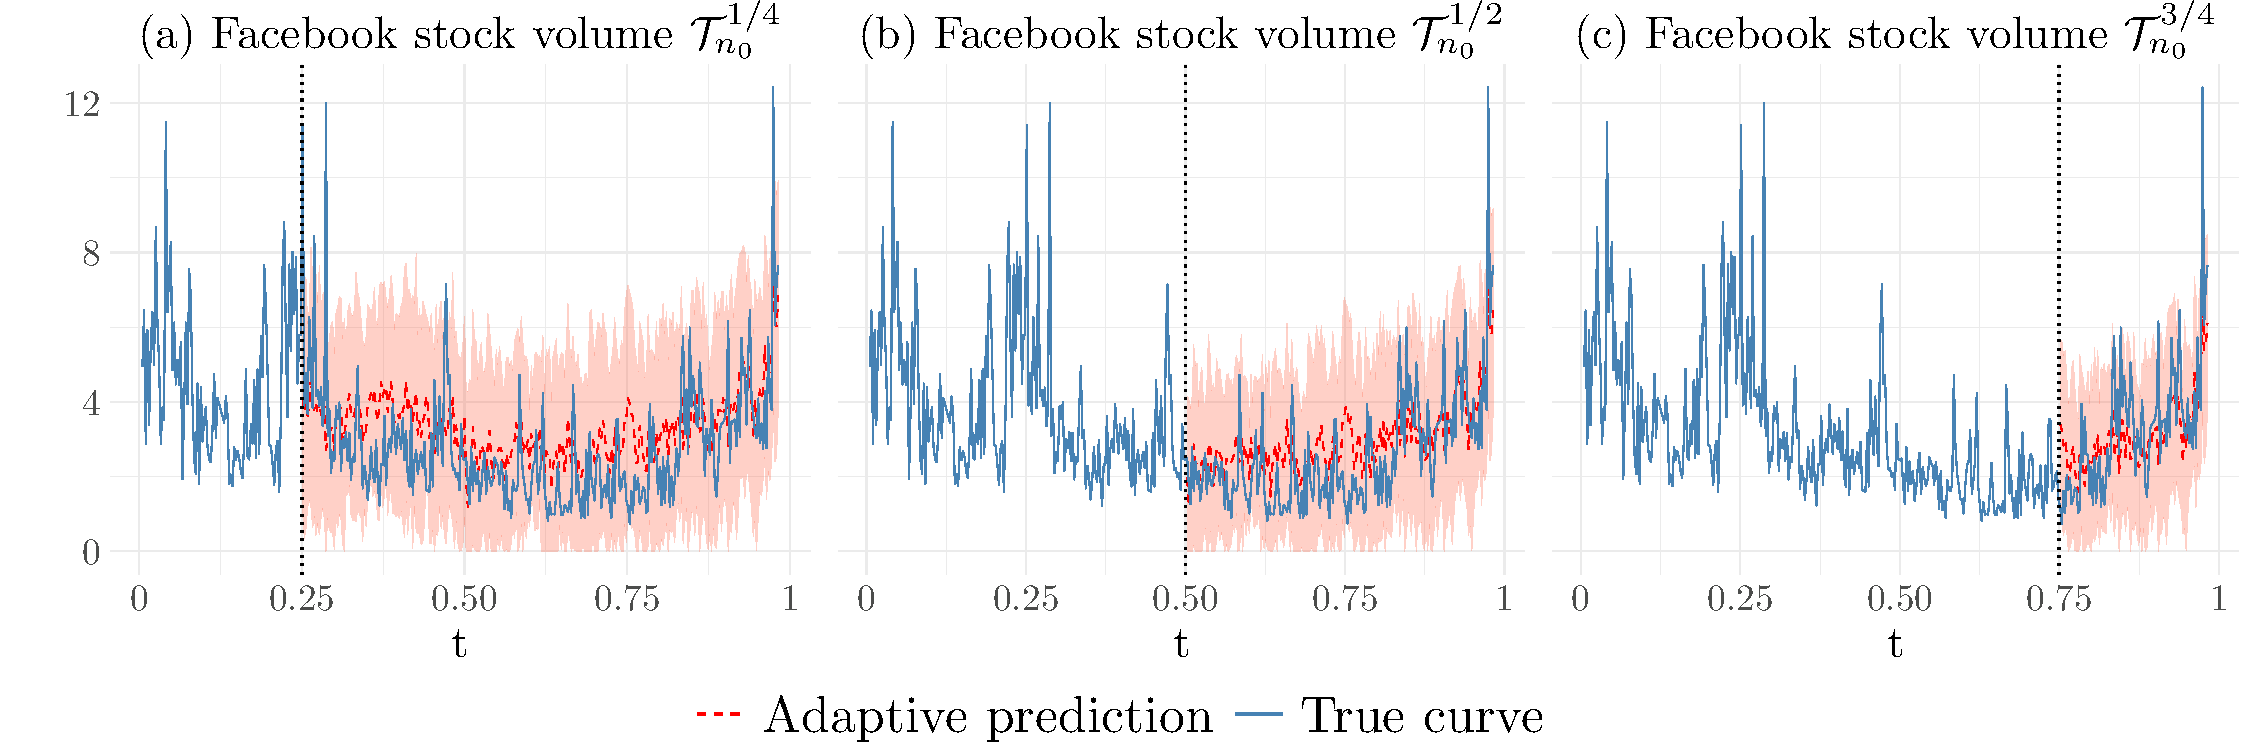
\includegraphics[width=\textwidth]{./figures/blup/Facebook_stock_volume_adaptive_pred_with_conf_band.pdf}
	\caption{\small Predictions of the last Facebook stock volume curve under scenarios where observations are available in $(0, 1/4]$, $(0, 1/2]$, and $(0, 3/4]$, respectively. The solid line shows the true curve, the dashed line shows the predicted curve, and the shaded band indicates the 95\% pointwise confidence interval. Stock volume values are normalised by $10^4$.}   
	\label{fig:facebook_real_data_blup}
\end{figure}



%%%%%%%%
%% Electricity forecasting
%%%%%%%%

%Forecasting electricity consumption and production is essential for maintaining the balance of the electricity system, as it helps to significantly reduce the costs associated with storage and overproduction. Accurate forecasting is therefore a major economic challenge, especially in sectors such as hydropower and photovoltaics, where production varies significantly throughout the day due to weather dependencies. Functional time series provide an effective framework for modelling such trajectories, especially when the forecasting method adapts to the regularity of the underlying process, as in the case of adaptive BLUP. 
%
%\begin{figure}[h]
%	\centering
%	
\includegraphics[width=\textwidth]{Chapitre3/figures/blup/plot_adaptive_blup_energy_with_conf_band.pdf}
%	\caption{\small Electricity curve prediction. The first row shows the results for the consumption curves, the second for the photovoltaic curves, and the third for the hydroelectric curves. Each column corresponds to reconstructing the solid curve with available observations restricted to the intervals $(0, 1/4]$, $(0, 1/2]$, and $(0, 3/4]$, respectively. The shaded bands indicate the 95\% pointwise confidence intervals.}   
%	\label{fig:real_data_blup}
%\end{figure}
%
%To illustrate this approach, we analyse daily curves of national electricity consumption in France, along with daily production curves for photovoltaic and hydroelectric electricity, obtained from the ODRÉ platform \citep{odre_data}. The dataset for consumption spans the period from June to September 2024 and comprises $122$ daily curves. Each consumption curve is recorded at $96$ equally spaced time points, with measurements taken every $15$ minutes. The photovoltaic production dataset also covers the period from June to September 2024 and includes $122$ daily curves. Since photovoltaic output depends on sunlight, observations are restricted to $61$ time points recorded every $15$ minutes between 4~a.m.\ and 7~p.m.\ on the same $122$ days. The hydroelectricity production dataset consists of $152$ daily curves observed at $96$ equally spaced time points every $15$ minutes, collected between November 2023 and March 2024. All values for each type of curve are normalised to the interval $[0,1]$ by scaling them with the maximum observed production value.
%
%To assess the empirical autoregressive structure, we estimate the lag-$1$ FACF using \eqref{eq:blup:facf}, obtaining values of $0.42$, $0.44$, and $0.36$ for the consumption, photovoltaic production, and hydroelectric production curves, respectively. These estimates provide evidence that the autocovariance-related blocks in $\VV_{n_0}$ are non-negligible, which indicates that the lagged curve contributes meaningfully to the adaptive BLUP. Moreover, each estimated FACF falls within the empirical distribution of lag-$1$ FACF values observed in our simulation study (see Figure~\ref{fig:conso_lag1_facf}).
%
%Figure~\ref{fig:real_data_blup} presents a comparison between the adaptive BLUP predictions and the actual curves to be predicted for the three types of curve sets, together with the 95\% pointwise confidence interval. The comparison is conducted under scenarios where the available observations are restricted to the interval $(0, \alpha]$, with $\alpha \in \{1/4, 1/2, 3/4\}$. Across all curve types and observation scenarios, the adaptive BLUP effectively captures local irregularities and demonstrates satisfactory predictive performance.



\FloatBarrier
